%!TEX root = ../thesis.tex
%*******************************************************************************
%****************************** Sixth Chapter **********************************
%*******************************************************************************
\chapter[CDI in Action]{CDI in Action: Applying the Model of CDI for Civic Advocacy and Action}
\label{chap:cdi_in_action}
% **************************** Define Graphics Path **************************
\ifpdf
    \graphicspath{{Chapter6/Figs/Raster/}{Chapter6/Figs/PDF/}{Chapter6/Figs/}}
\else
    \graphicspath{{Chapter6/Figs/Vector/}{Chapter6/Figs/}}
\fi

\epigraph{If you do not know how to ask the right question, you discover nothing.}{--- \textup{W. Edwards Deming}}

This chapter focuses on understanding the challenges of making data \textit{useful} for the community and the methods that may help guide people through the whole process of achieving the effective use of data to support civic advocacy and action. Using the model of CDI established in the previous chapter, this chapter presents a case study where the model was applied in practice. Building on the practical approaches set up in the previous chapter (Section \ref{sec:pract_cdi}), a dual approach was taken to work on the engineering problem-solving agenda as well as the community problem-solving activities of CI, which included a redesign of the Data:In Place platform; the use of hypothesis setting and leveraging Right Question Institute's (RQI)\footnote{\url{https://rightquestion.org/}} Question Formulation Technique (QFT) to aid people to better articulate their questions for data; and the use of challenge creation to help people come up with strategies towards action that make effective use of data. The case study was conducted through running data consultations in focus groups with key stakeholders from an NPO and through a Community Action Day with the local community in a workshop setting, where a combination of digital tools with supporting methods were trialled to address the dual agenda of CI. All the participants involved in the case study also took part in the initial design processes of Data:In place, as described in Chapter \ref{chap:datainplace}. The present chapter begins by highlighting the challenges and motivation for this study and explaining the dual approach in the context of CDI to apply this in a two-phase study, where two communities are trying to make effective use of data. In addition, the chapter presents empirical evidence regarding the use of CDI and the effectiveness of these methods to define actionable steps towards purposing data, in addition to starting to map out the supported processes needed for the effective use of data in advocacy and action, processes that have often been neglected by designers and information engineers building automated information technologies (AIT) for data discovery.
\clearpage

\section*{Related Publications and Acknowledgements}
\begin{itemize}
\item Acknowledgements go to Dr. Jan Smeddinck for helping with the research design of the study and Thomas Maskell for helping to run the community workshop activities.
\end{itemize}
\clearpage

\section{Motivations}
Developing and deploying tools that promote better \textit{access}, \textit{comprehension} and \textit{usability} of data does not mean that the data will find its way into actionable results. Data itself is not evident or inherently useful \citep{gitelman_raw_2013} to a person or group who is able to access it. In both case studies, SMS (Chapters \ref{chap:sensemystreet} and \ref{chap:sensemystreet-eval}) and Data:In Place (Chapter \ref{chap:datainplace}), the technologies built aimed to make data more accessible by anchoring it with place and local context so that people could make sense of it. With SMS, it was a case of democratising \textit{data production}, whereas with Data:In Place, it was a case of democratising \textit{data access}. Both studies made good progress towards helping people access and explore different datasets on their own terms. However, they might also have created an overload of choice for people rather than helping them come up with questions, queries and strategies for data use. From the case studies, it became evident that it is not only up to engineers to build better tools and interfaces for data, but there are also other, more human, factors that need to be explored to combine a more holistic approach for the effective usage of data in civic action. As a result, a model of CDI was proposed to illustrate the key elements of effective use of data by communities.

The case study builds on previous work conducted in this thesis related to community data production using the SMS commissioning platform (Chapter \ref{chap:sensemystreet}) and exploring the uses of OGD for local decision-making using the Data:In Place platform (Chapter \ref{chap:datainplace}), combining the knowledge gained from designing, developing, deploying and evaluating these data systems. Extending on the previous case studies and using the model of CDI, this chapter discusses what makes people go from `I want to see all the data' to `I want to see data that relates to a question I have', thus providing data for an actionable purpose. Such issues link to the open challenges set out in the previous chapter (Section \ref{sec:new_challenges}) that need to be addressed around CDI to enable the effective use of data by communities. Building on the previous chapter's practical approaches (Section \ref{sec:pract_cdi}), this chapter explores how we might start linking data to questions that people have and actions they want to take. Through the use of CDI and the dual approach, this case study aims to improve the processes of inquiry for data by applying digital technologies and cognitive processes to use data in support of civic action in complex sociotechnical settings.

\section{Dual Approach for CDI}
\label{sec:dual_cdi}
The case study follows the overall approach of PADRE utilised in this thesis \hyperlink{introduction}{Introduction}; however, to address the open challenges of CDI arising from the previous case studies, a more holistic approach was taken. In this regard, an adopted version of the dual approach (Section \ref{sec:pract_cdi}) was taken to improve the ways people make requests for data and use strategies to help local communities deal with specific isolated questions. This was realised by working closer with communities to implement a set of \textit{mutually supporting strategies} (both technical and social cognitive) within the scope of and across two components, which included \textit{Component 1} -- systems approaches to promote the usage of data and build support for data discovery and \textit{Component 2} -- capacity building to make data actionable and increase a community's social capital to take action. This approach simultaneously focuses on technical implementations that can be used by everyone who has access to the internet and social cognitive strategies that focus on specific communities. In terms of CDI, the dual approach aims to address issues in all five key elements of the model. Table \ref{tab:dual_approach} illustrates the usage of dual approach strategies applied concurrently for improving general approaches to working with and using data, focusing on specific targeted communities to make data actionable. The general interventions are linked to new technical features integrated into the Data:In Place platform, and targeted interventions are methods to help local communities understand their data needs and plan actions for data. Both also include ways that the community can increase its social capital and create new links outside its immediate community. The following sections will go into more detail about the different types of interventions shown in Table \ref{tab:dual_approach}.

\begin{table}[!htb]
\scriptsize
\centering
\begin{tabular}{|l|c|c|c|}
\hline
\textbf{Component} & \textbf{Strategy} & \textbf{General Interventions} & \textbf{Targeted Interventions} \\ [0.5ex]
\hline
\rowcolor[gray]{.9}\textbf{System Approaches}	& \makecell{Build support for scalable accessing \\ and discovery of datasets} & Anchored Data Requests & Hypotheses, QFT \\
\hline
\textbf{Capacity Building} & \makecell{Improve effective use \\ and actionability of data} & Data Challenges & Challenge creation method \\ [0.5ex]
\hline
\end{tabular}

\smallskip\centering
    \footnotesize\emph{Source: Author}
\caption[Dual Approach for CDI]{Strategies for a dual approach in the context of CDI}
\label{tab:dual_approach}
\end{table}

\subsection[General Interventions]{General Interventions: The Redesign of Data:In Place}
\label{sec:data-in-place_redesing}
The initial prototype of Data:In Place (Chapter \ref{chap:datainplace}) was built to enable community groups and charities access and make sense of open data related to their local area. The design and development of the platform was largely driven by the questions and issues of a specific public, and the datasets that were first integrated into the system were a direct response to issues and questions posited by the local Neighbourhood Planning Group at their meetings. Furthermore, additional datasets were added through engagement with local charities and looking into ways their work could be targeted and evidenced. In later stages of the study, a \textit{Data Request Feature} was added to the system (Chapter \ref{chap:datainplace}) that enabled people to put in requests for datasets digitally, without having to meet face-to-face with a researcher, making it more generic for everyone to request adding datasets. Although that solved the issue of physical presence, it did not make it easier for people to come up with requests or for the researcher to reply to them. All these issues added to the core issue of the open datasets being underutilised by communities. The Data:In Place platform was facing the same issues that were pointed out in the case of the What Do They Know website (Chapter \ref{chap:cdi}).

Working on the dual approach's \textit{general interventions} meant improving the platform to help unpack the challenges around connecting people's questions and issues to abstract datasets. Additional features were implemented into the platform that automatically added contextual data to requests, with the aim of improving data responses to people's issues and questions. These took the form of \textit{anchored data requests} and \textit{data challenges}, which will be described in the following subsections.

\subsubsection{Anchored Data Requests}
\label{sub:anchour_requests}
The Data:In Place case study (Chapter \ref{chap:datainplace}) illustrated that to make data accessible and usable by people, it needs to be made relevant to place, local issues and local activities in order for it to become useful. These can be seen as anchors for data that make abstract datasets more comprehensible to people. However, using anchoring can also be beneficial when requesting new datasets to be added to the platform, providing contextual information to better understand the context where data needs to fit and be made use of.

The platform's \textit{data request} form provided people text entries for describing the issue they were exploring, linking the actual dataset or public authority who might posses the data and describing the issue by means of a story (Chapter \ref{chap:datainplace}). This works well if a person has an idea about what type of data they are looking for and how to access it. Then, it was a case of connecting the database with the map-based querying of Data:In Place. Furthermore, if the particular data provider used standardised vocabularies and descriptions of the data (such as linked data or JSON-LD) exposed through an API, these processes could be further automated. However, if a person had no idea what data might be useful for exploring a particular local issue, it made it much more difficult for the researcher to find those datasets to add to the platform. Previous work undertaken in this thesis on developing the Data:In Place platform (Chapter \ref{chap:datainplace}) within the context of the neighbourhood plan illustrated that people had difficulty making connections between particular issues and datasets that might inform them. They had an understanding that there might be some data available, e.g. by making a statement that `the council has the data'; however, the type and format of the data was unknown to the community. Working closely with the community and attending their neighbourhood plan meetings enabled the author to make these connections because of the added context obtained from these meetings. This again points out the heavy reliance on the work of data professional to make these connections and find the data needed.

To improve data requests on the Data:In Place platform and add additional context alongside the submissions, a metadata collection was implemented that included map \textit{boundary data} (Chapter \ref{chap:datainplace}) drawn by the request submitter, the submitter's \textit{geographical location} (provided it was allowed by the person) and the previously \textit{explored datasets} within the submission session. This additional metadata, which was automatically attached to the requests, provided some of the context that would have originally been obtained through the community engagements but was missing when people only interacted with the system, and it could potentially help respond to requests with more accurate and useful datasets for the community.

\subsubsection{Data Challenges}
\label{subs:data_challenge}
An issue encountered in both the previous case studies (Chapters \ref{chap:sensemystreet} and \ref{chap:datainplace}) was the lack of action in regard to using the data once it had been obtained. This was often an issue of not possessing the skills needed to work with the data in order to transform it into something usable (Data:In Place Chapter \ref{chap:datainplace}); however, it also related to the lack of planning or mapping out routes to actions that would be of local benefit. This meant developing attachments to the data and committing to activities that would use it. These issues are tightly coupled with building community capacity and reaching out to supporting networks for additional support and skills, which is a big part of the CDI model. Some of these processes could be automated, but it was still evident that, in some cases, people would need support from professionals.

As a response, a \textit{Data Challenges} feature was added to the platform, which enabled people to post challenges about \textit{finding}, \textit{accessing}, \textit{producing} and \textit{making sense} of data, in addition to then \textit{taking action} with it. This served two purposes: first, to serve as a plan for taking action with data (i.e. making data useful), and second, as a way to increase the capacity and widening the community network by reaching out to people externally. Technical features that were added were: a Markdown\footnote{\url{https://www.markdownguide.org}} form and tagging functionality for submission forms (Figure \ref{fig:chall_form}), resulting in a data challenge info display (Figure \ref{fig:chall}). These types of technologies are commonly used for issue reporting on software development platforms such as GitHub\footnote{\url{https://github.com}}. Furthermore, the same metadata was collected and added to the \textit{Data Request} forms, enabling a direct link to be made to the challenge (Figure \ref{fig:chall_link}). Additionally, a \textit{focus bar} was added to the platform to always display the aim of the investigation when a particular challenge was selected. This focus bar also served the purpose of providing an issue focus in the \textit{question-asking} activity in community workshops (Section \ref{sub:qft_action}).

\begin{figure}[ht!]
\centering
 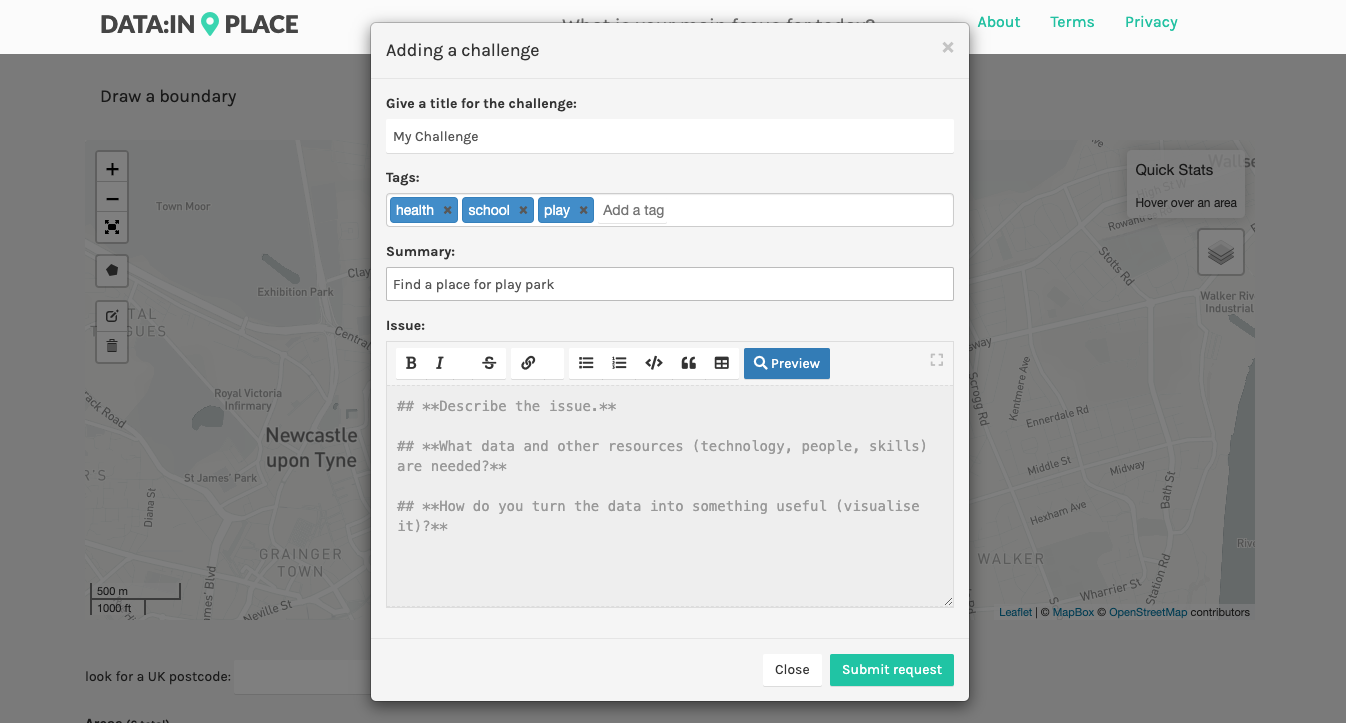
\includegraphics[scale=0.3]{make_challenge}
  \caption[Data Challenge Form]{Screenshot of data challenge form}
  \label{fig:chall_form}
\end{figure}

\begin{figure}[ht!]
\centering
 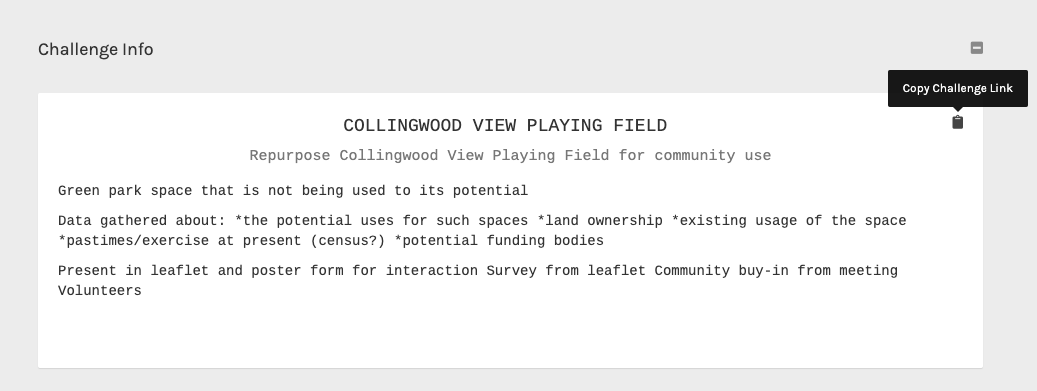
\includegraphics[scale=0.3]{challenge}
  \caption[Data Challenge]{Example of a data challenge}
  \label{fig:chall}
\end{figure}

\begin{figure}[ht!]
\centering
 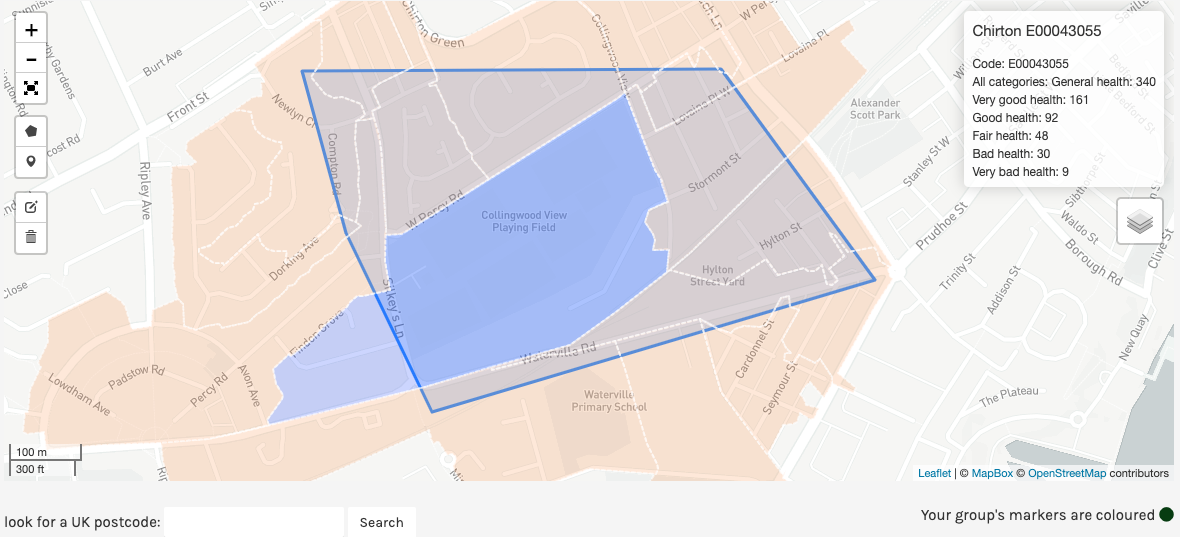
\includegraphics[scale=0.3]{challenge_link}
  \caption[Data Challenge Link]{Example of a data challenge link}
  \label{fig:chall_link}
\end{figure}

\subsection{Targeted Interventions}
\label{sec:targeted_engagements}
In addition to focusing on the technical implementations by adding features on the Data:In Place platform, a parallel more targeted approach was also taken to aid people in making data useful for their purposes. This consisted of engagements with different groups of people interested in using data in community settings to explore or evidence issues and take action. This was carried out by guiding people in positing better questions for data and assisting in the creation of steps for actions based on the data. In addition to directly working with these communities and providing them professional support, the aim was also to develop methods and resources that could be used to help other people outside these communities use the new features of the Data:In Place platform and find actionable use for data.

\subsubsection{Hypotheses}
\label{sub:hypotheses}
In order to know what types of data are needed or might become useful for a particular case, there needs to be a clear aim for the investigation. The case studies described in the previous chapters, although both working with different communities and datasets, had a recurring criterion for the successful use of data in action -- data was found useful in civic action only when people knew ahead or planned out what they were looking for in the data, i.e. when they were asking the right questions from the data. Having a predefined agenda for the use of data turned out to be particularly important for community groups who were hoping to use data for civic action. This was also illustrated by the CAF in (Chapter \ref{chap:sensemystreet-eval}). However, setting that agenda was a difficult cognitive task, which often required the knowledge of a professional data analyst. In a sense, it was a `chicken and egg' dilemma that needed further investigation in order to depict the variables that influence the process of discovery and queues that would aid people in coming up with these agendas.

A common practice in scientific research projects is to first start with hypotheses that the projects are trying to prove (alternative hypothesis) or disprove (null hypothesis). This approach is used in a variety of scientific communities and fields, from engineering to social sciences, which forces one to come up with a set of statements to explain a phenomenon or process. Hypothesis setting and investigation was one of the approaches trialled in the case study with participants from Charity A, who were not professional data analysts, to develop statements for discovering and making use of data.

\subsubsection{Question Formulation Technique}
\label{sec:qft}
The scientific hypothesis approach or scientific approach may work in professional settings with people who are familiar with these concepts. However, the aim of this thesis is to help truly democratise these practices and make them work in community contexts where the scientific approach is not commonplace and most probably would not work. To make the process more inclusive and not serve the values of some stakeholders over others, there was a need to look at additional, alternative approaches. The closest things to hypotheses are questions, which people ask every day. The difference is that the questions are unknown and highly dependent upon the context and the way they are formulated.

The challenge was to come up with questions and issues that could be mapped to and explored by means of abstract datasets. There was a need for a better process of guiding people in asking questions that could be explored and answered using data. Fortunately, there was already an existing process, the QFT, which was initially developed by the RQI\footnote{\url{https://rightquestion.org}}, to assist parents in better participating in their children's education process so as to prevent school dropouts. Furthermore, RQI's methods have now been used in a variety of contexts and settings, such as education, health and social care, community-based organisations, and in local democracy. In general, the aim of RQI strategies is to \textit{`help all individuals learn how to ask better questions, participate more effectively in decisions, advocate for themselves, their families, and communities, and hold decision-makers accountable on all levels of democracy'}\footnote{\url{https://rightquestion.org/what-we-do/}}. The QFT strategy, in particular, is a guided step-by-step process to helps people formulate, improve and use their own questions by applying multiple ways of thinking: (i) divergent thinking -- linear learning and following instructions; (ii) convergent thinking -- generating one's own problems and questions; and (iii) metacognitive thinking -- reflecting on one's own cognitive processes. The detailed process of the QFT is summarised in Figure \ref{fig:qft}.

\begin{figure}[ht]
\centering
 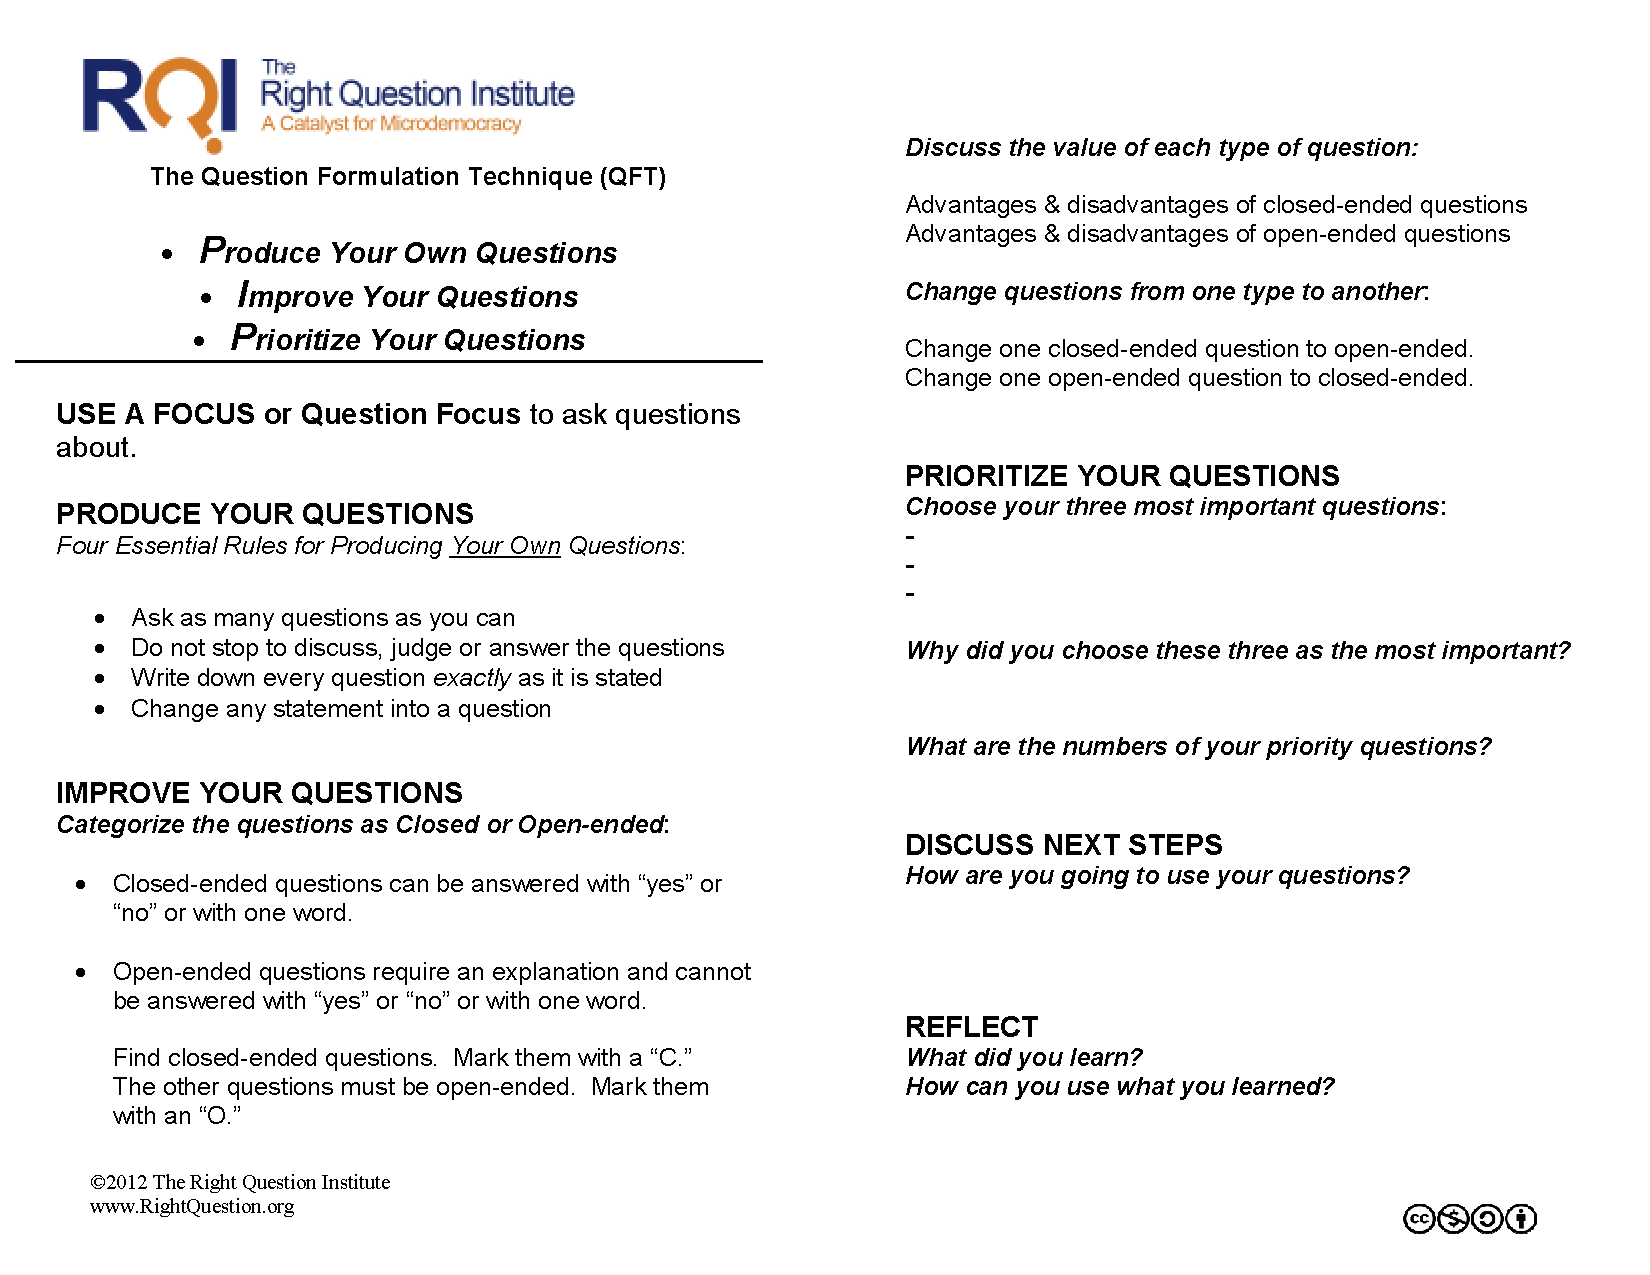
\includegraphics[width=\linewidth]{QFT-Card-Template}
 \smallskip\centering
  \footnotesize\emph{Source: \url{https://rightquestion.org}} 
\caption[Question Formulation Technique]{Question Formulation Technique (QFT)}
\label{fig:qft}
\end{figure}

\subsubsection{The Challenge Creation Method}
Asking the right questions may help people better \textit{access}, \textit{interpret} and \textit{make sense} of the data used in decision-making processes and perhaps even collect their own data to inform an issue. However, to effectively participate in these processes using the same data, people need to be able to come up with plans or strategies for civic action that \textit{make use} of these datasets. A more in-depth approach had to be taken to explore and map out the steps that people need to take to move from questions and statements to planning out actions for data. Creating plans for action needed to integrate questions and statements as the starting point and get people thinking about the practical steps that needed to be taken to answer them. This also included figuring out what type of data might be useful and in what form and what kind of resources were needed to make it happen. This guiding process was called \textit{challenge creation} so as to link it with the general intervention approach of submitting data challenges (Section \ref{subs:data_challenge}).

The next section describes the study design taken to investigate the effectiveness of these approaches, accompanied by the general intervention strategies described in Section \ref{sec:data-in-place_redesing}. This includes planning data consultation focus groups for hypothesis setting, leveraging \textit{Ambit} \citep{johnson_creating_2020}, a tabletop game for mapping and reflecting on issues, creating a modified approach to the QFT method to help people come up with questions that can be answered by exploring different datasets, and integrating challenge creation guides with QFT to be trialled in community setting. The aim of applying these methods in a workshop setting with a specific population was to enable people to make better use of Data:In Place's added features for data use (Section \ref{sec:data-in-place_redesing}) that were part of the general interventions of the dual approach. In terms of CDI, these interventions are part of \textit{social facilitation}, enabling an increase of capacities and utilising infrastructures to use data effectively.

\section{Study Design}
\label{sec:cs3_design}
The evaluation of the case study methods and processes were undertaken in two subsequent phases:

\begin{itemize}
\item[PHI.] (\textit{Data Consultations}) involved running focus groups with key stakeholders from a large local charity (Charity A) organisation funded by many local organisations and lottery funds. Charity A worked on programmes and interventions around the health and wellbeing of young people, and they were also involved in the design of the Data:In Place platform (Chapter \ref{chap:datainplace}). Data consultations were run in a format where the author acted as professional support for the participants in regard to exploring and purposing datasets. This phase served as initial scoping to understand the cogitative processes that people go through in order to come up with actionable strategies for data use. Additionally, focus groups provided requirements for the further design of the Data:In Place platform.

\item[PHII.] (\textit{Community Action}) focused on the evaluation of methods for helping people formulate better questions for data and deriving challenges from those questions. This phase built upon PHI and was conducted through a workshop where multiple methods were coupled to help participants explore and identify issues, posit problems and questions, and plan actions for utilising data in community context for civic action. Participants involved in this study were residents from the same local community who were participating in the neighbourhood planning meetings and the initial design of the Data:In Place platform (Chapter \ref{chap:datainplace}).
\end{itemize}

Figure \ref{fig:cdi_phases} illustrates the two phases of the case study and the digital tools and methods used to explore ways to help people make effective use of data. The process consisted of five stages: identifying \textit{issues}, setting \textit{focus}, asking \textit{questions}, creating \textit{challenges}, and taking (or planning) \textit{actions}. Furthermore, the figure outlines the important elements in each stage of the process that either acted as anchors or were considered as objects of change. Through these study phases, the following questions were explored:
\begin{enumerate}
 \item How can people articulate the questions they are asking about the data?
 \item Dual approach for CDI:
 \begin{enumerate}
    \item How to citizens transform data into something valuable (i.e. make data useful)?
    \item What is the real value for citizens accessing these datasets?
 \end{enumerate}
 \item Roles in CDI:
 \begin{enumerate}
      \item What role will non-professionals and (semi-)/professionals play in this?
      \item What would the collaboration between professionals and non-professionals look like?
 \end{enumerate}
\end{enumerate}

\begin{figure}[!htb]
\centering
 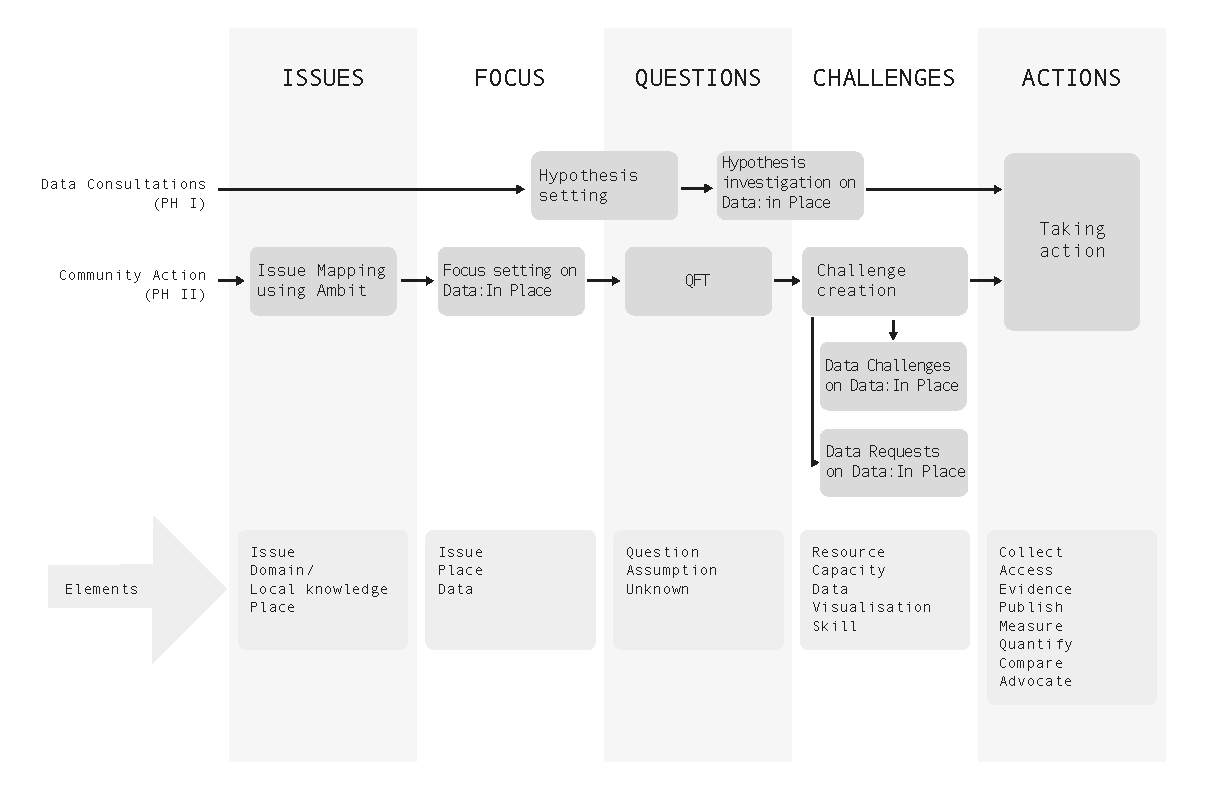
\includegraphics[width=\linewidth]{study_phases}
 \smallskip\centering
  \footnotesize\emph{Source: Author}
  \caption[CDI Study Phases]{Tools and methods used in different study phases across the five stages of making data useful}
  \label{fig:cdi_phases}
\end{figure}

\subsection{Apparatus}
\subsubsection[Issue Mapping]{Issue Mapping: CC in Community Action}
CC is a method developed by \cite{johnson_community_2017} that uses \textit{Ambit} \citep{johnson_creating_2020}, an augmented reality audio capture tool build in Open Lab at Newcastle University to support deliberation in consultation processes for local decision-making in community settings. It has proved to be a valuable tool to structure the process and document the voices of people who traditionally would have not been included in these processes, making the process more inclusive and democratic \citep{johnson_community_2017,johnson_neighbourhood_2018}. A modified version of CC (CCmod) was trialled\footnote{CCmod was designed in collaboration with Dr Ian Johnson and the author and built by the author.} in Case Study II (Chapter \ref{chap:datainplace}) to map local issues and gather people's opinions about them \citep{johnson_neighbourhood_2018}. The location-based opinion data gathered through this process was then fed into the Data:In Place platform (Section \ref{chap:datainplace}) as another datasource generated by citizens themselves open for interrogation, side by side with official open datasets.

\begin{figure}[!htb]
\centering
 \includegraphics[scale=0.1]{ccv2}
  \caption[Community Conversational Map]{Modified CC map for Ambit technology with pre-marked locations}
  \label{fig:ccv2_cards}
\end{figure}

The workshop made use of the data gathered in previous workshops with the participants (Chapter \ref{chap:datainplace}) to start off with a set of issues that had been previously identified by the community. Figure \ref{fig:ccv2} shows the CCmod map used in the workshop, with pre-marked locations from previous sessions. The issue marking activity followed the mechanics of CC (Chapter \ref{sec:datainplace}); however, a new set of prompt cards (n=2) were created to give more focus to the community action workshop: (1) \textit{wild card}, which enabled a new location or new information about a previous location to be added and (2) \textit{second that}, which enabled people to prioritise markers that had set a focus on issues. Additionally, participants in each group had a limited set of turns to add things to the map due to the time constraints of the workshop. This was determined by additional stickers on the cards that they had to place on the map, as shown in Figure \ref{fig:ccv2_cards}. 

\begin{figure}[hbt!]
\centering
 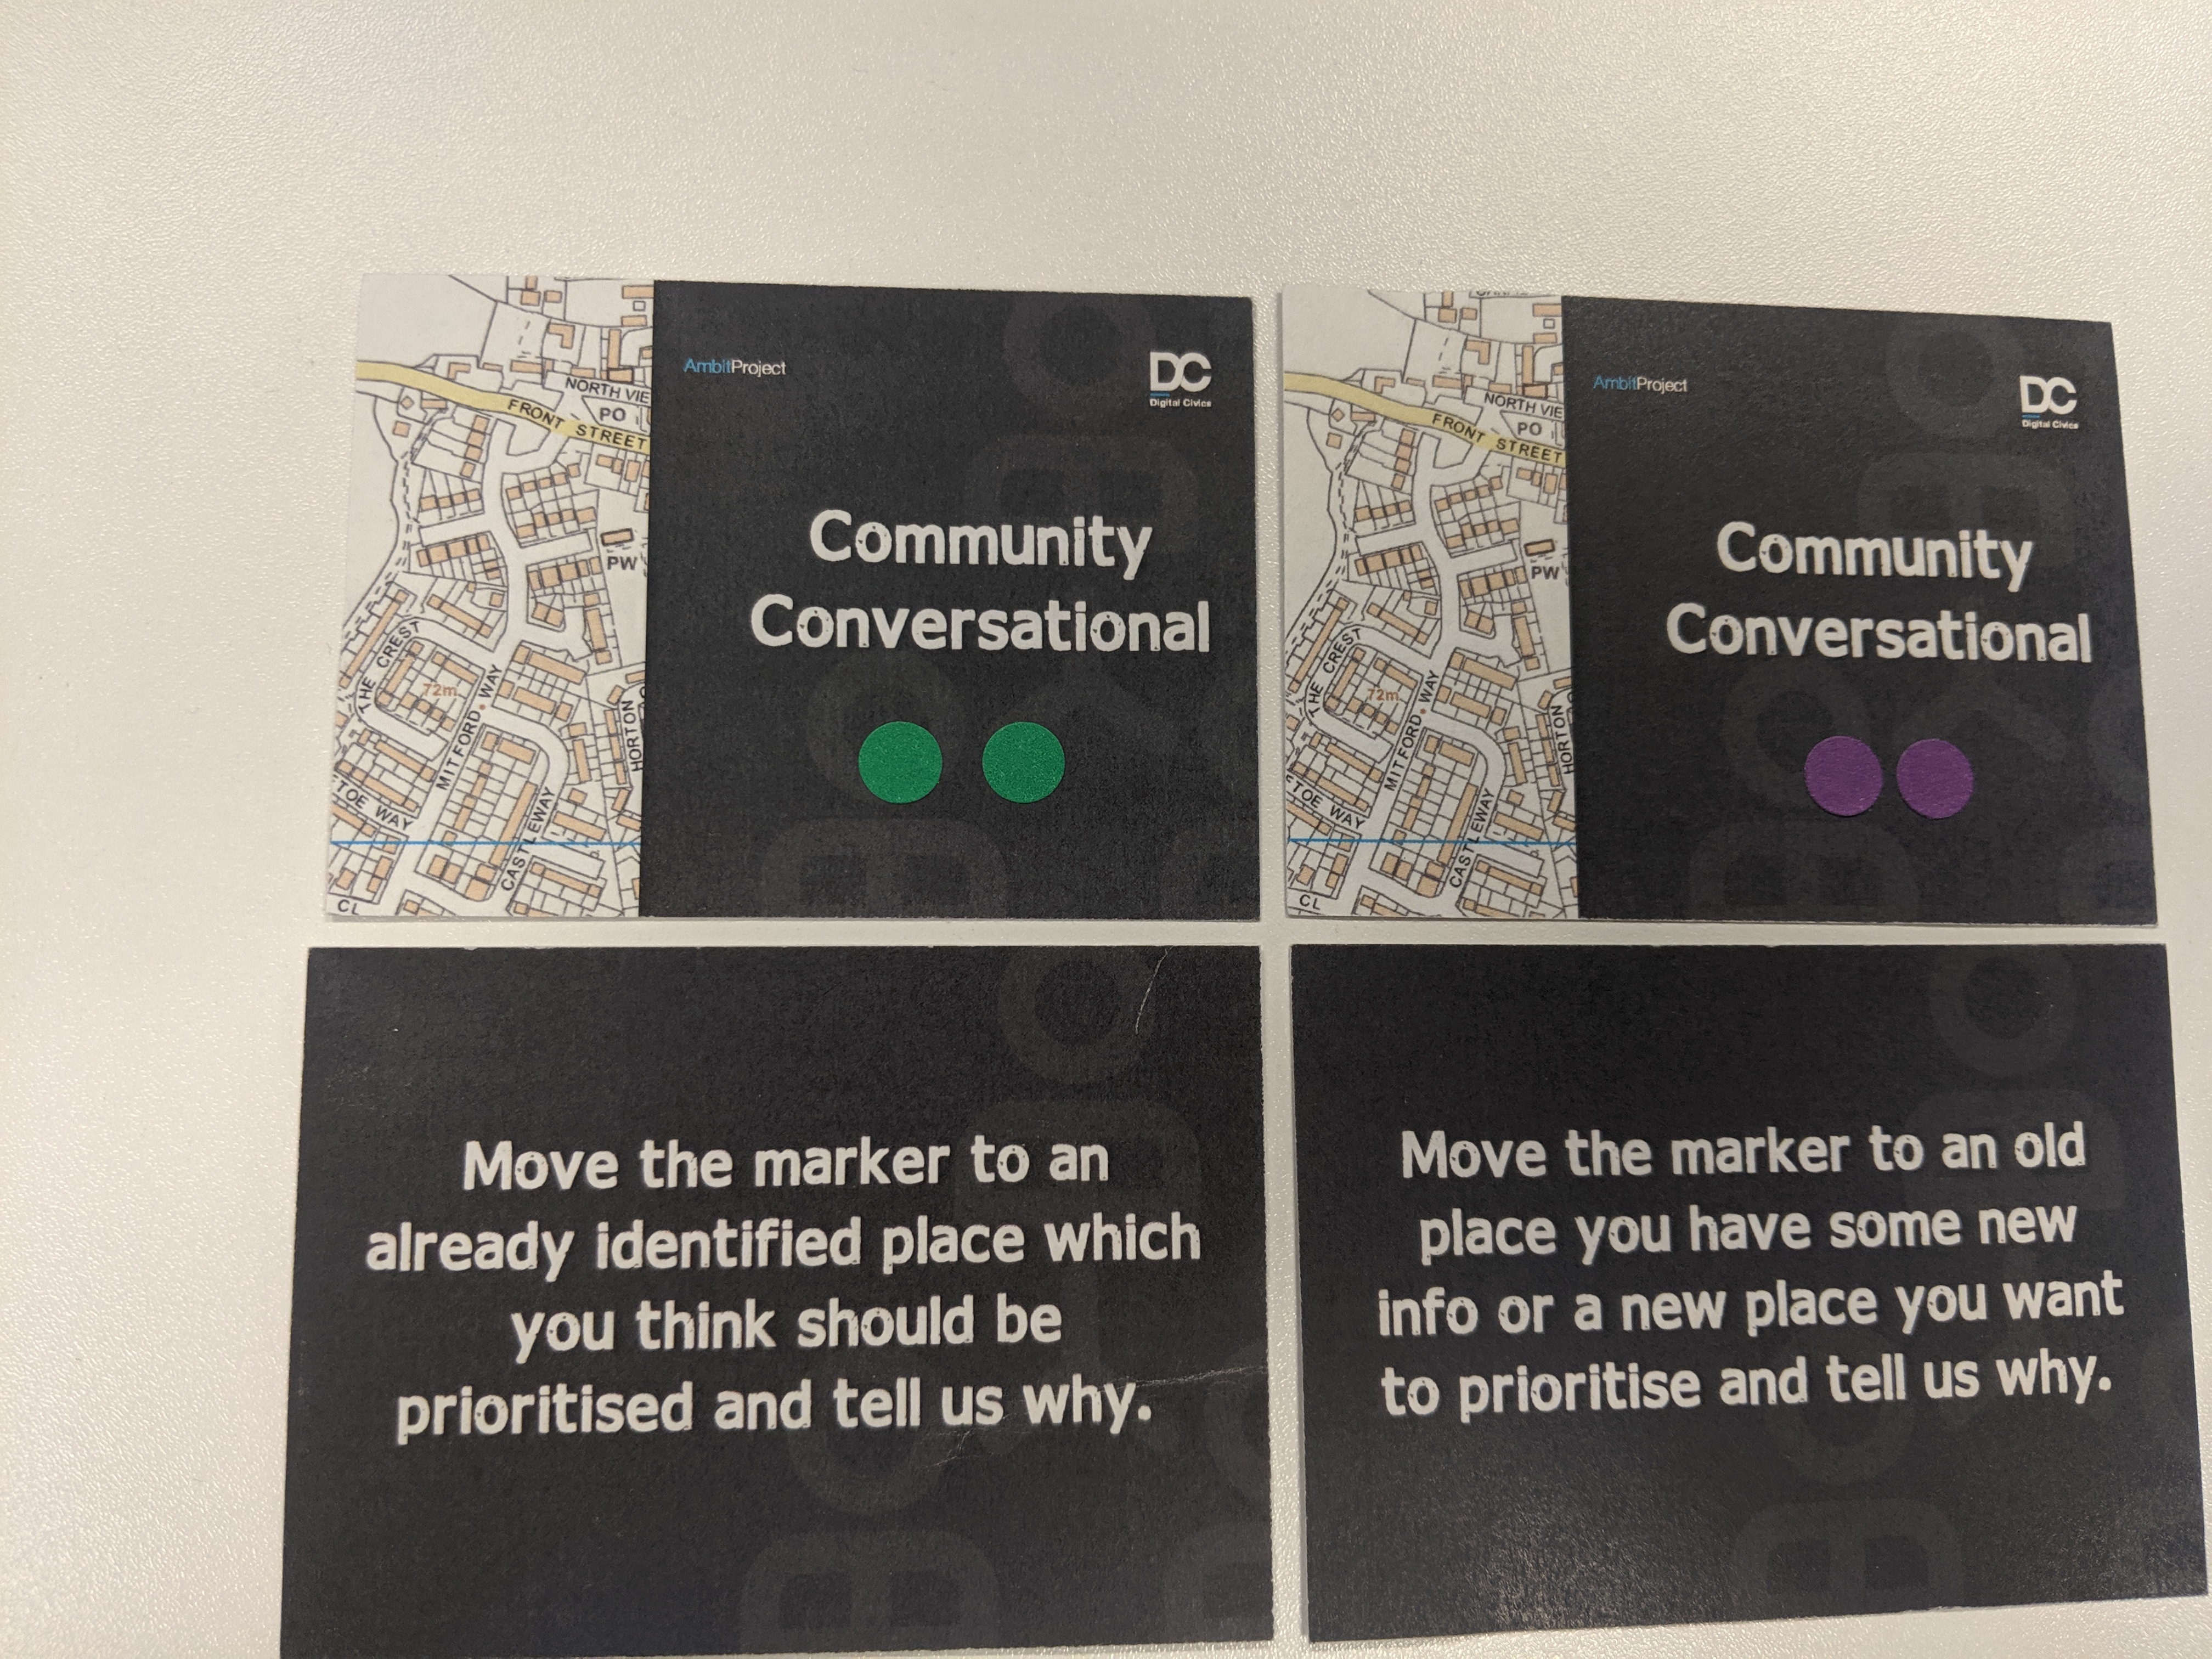
\includegraphics[scale=0.1]{ccv2_cards}
  \caption[Community Conversational Cards]{Modified CC cards}
  \label{fig:ccv2}
\end{figure}

\subsubsection[Focus Setting]{Focus Setting: Data:In Place in Community Action}
The second activity used in the community action workshop following the \textit{issue mapping} was \textit{focus setting}, which built on the mapping exercise to help the group focus on a specific issue. Groups had to choose an issue from the map that had the most support and consolidate that issue using the Data:In Place interface. In addition to discussions in the group, people could also use the Data:In Place platform to listen to location-based recordings from previous sessions recorded using Ambit (Chapter \ref{chap:datainplace}). After the group reached consensus through discussing and listening back to previous opinions, they used a mapping functionality to mark the issue on a map, similar to how they had done previously on the paper map. Issue mapping was a new feature that was specially built and added for running the community action workshops.

\begin{figure}[!ht]
\begin{subfigure}{0.32\textwidth}
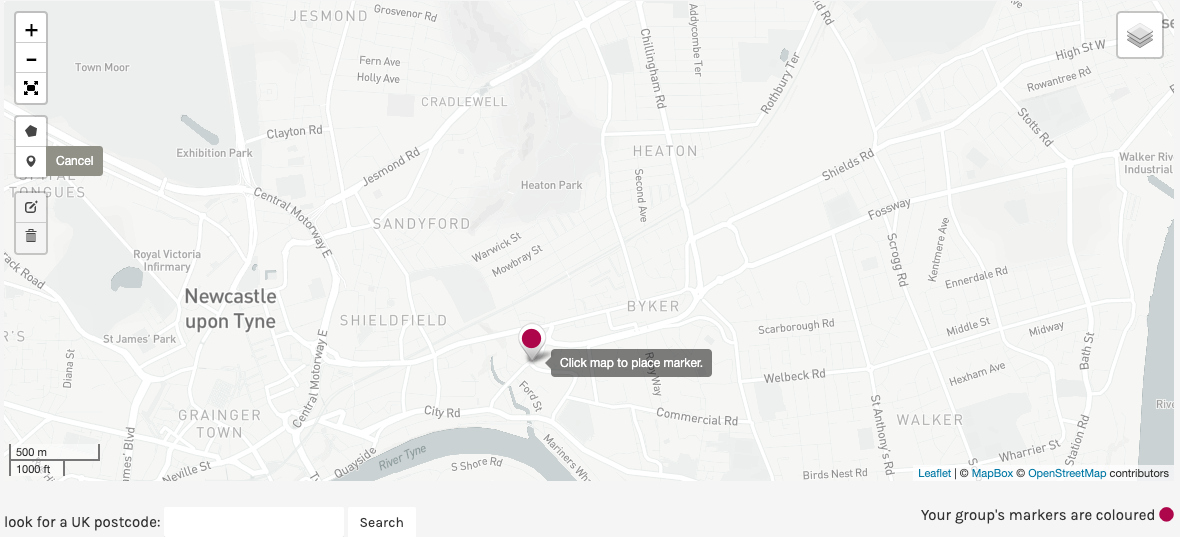
\includegraphics[width=\linewidth]{issue_1}
\caption{Group 1 locates a place for an issue} \label{fig:issue_1}
\end{subfigure}
\hspace*{\fill}
\begin{subfigure}{0.32\textwidth}
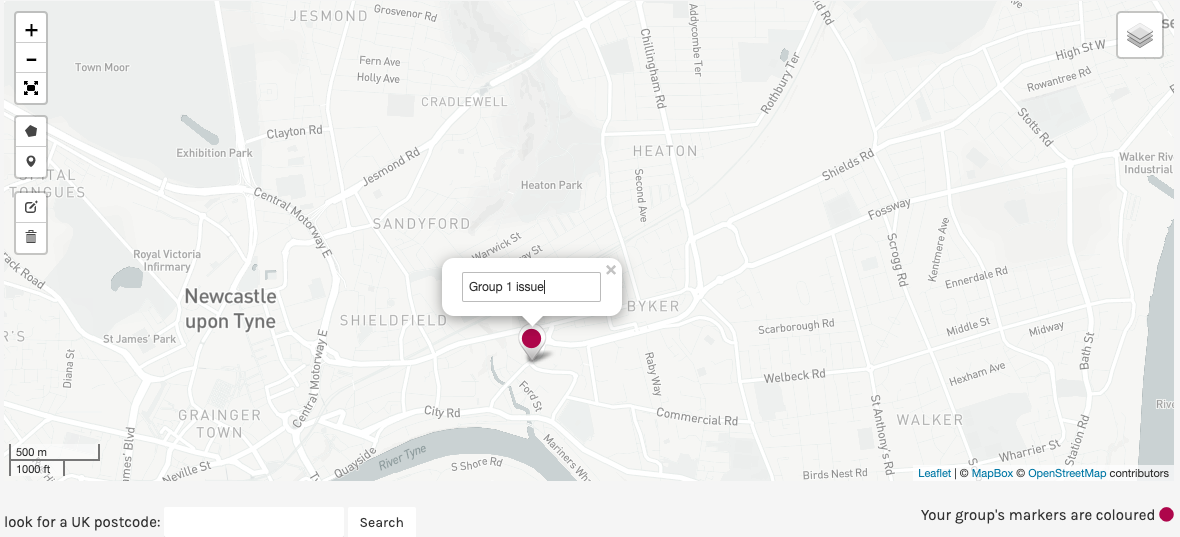
\includegraphics[width=\linewidth]{issue_2}
\caption{Group 1 maps and describes an issue} \label{fig:issue_2}
\end{subfigure}
\hspace*{\fill}
\begin{subfigure}{0.32\textwidth}
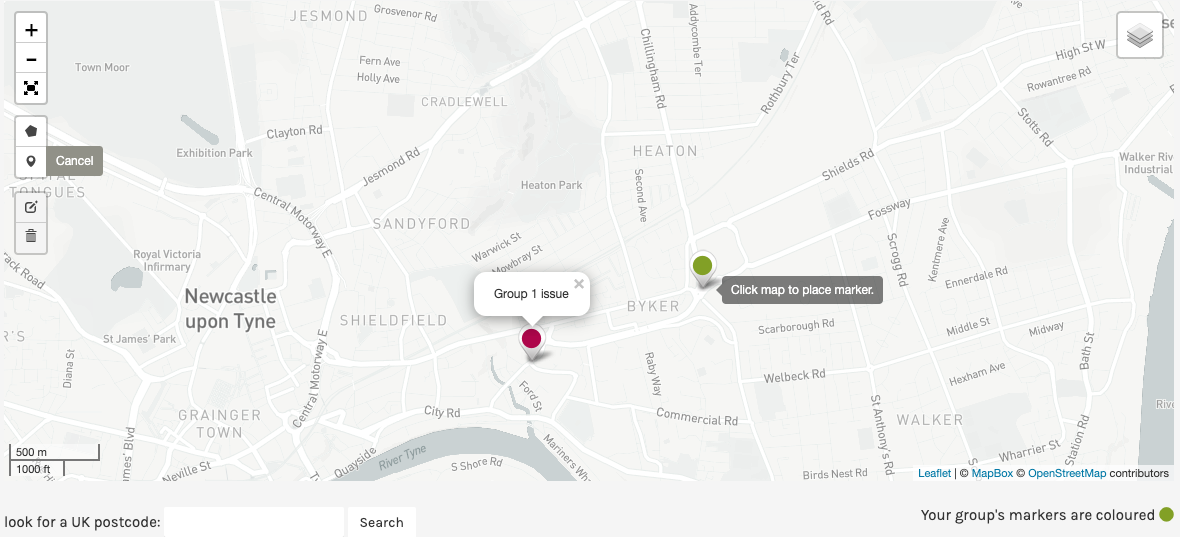
\includegraphics[width=\linewidth]{issue_3}
\caption{Group 2 sees Group 1 issue and can map their own} \label{fig:issue_3}
\end{subfigure}
\caption[Focus Setting]{Issue focus workflow} \label{fig:issue_prior}
\end{figure}

One other added feature integrated into the Data:In Place platform for the workshop was a \textit{live map view} using WebSockets\footnote{\url{https://developer.mozilla.org/en-US/docs/Web/API/WebSockets_API}}, which enabled the participants to see what other groups were doing on the map in real time, thus promoting reflection and collaboration. This also guaranteed that the groups would work in different areas and on different issues, covering more ground. A workflow of focus setting in a two-group session is illustrated in Figure \ref{fig:issue_prior}. All the data inserted into the Data:In Place system was saved for further analysis and recall, which includes boundary data, mapped issues and their geographical coordinates.

\subsubsection[Question Asking]{Question Asking: QFT in Community Action}
\label{sub:qft_action}
The third method used was the QFT, which was appropriated as a design interaction method in a workshop setting for helping people find uses for data in community action. Previous activities helped to feed into the QFT method by setting a focus for the question asking (Figure \ref{fig:qft}). The QFT had already been used in multiple contexts; however, it had never been trialled as a design method in PADRE and was a novel engagement method in HCI. This part of the community workshop was run as a guided exercise, where the QFT was explained step-by-step using an example of `rock climbing' (chosen by the thesis author). Additional worksheets were made and given to the participant on each of the steps (Appendix \ref{app:community-action}), which were new configurations of the original QFT worksheets (Figure \ref{fig:qft}), to make them more focused on community action. This guaranteed that the participants followed the structure of the method, keeping participants focused on only one task at a time and making the assessment on each stage easier. As a result of this activity, people had a top priority question that they selected as a group from a pool of questions created by leveraging the QFT method.

\subsubsection{Challenge Creation in Community Action}
The final method used in the community action workshop was \textit{Challenge Creation}. In the context of the effective use of data, a \textit{data science challenge} falls under categories such as data access, collection, data processing and analysis, augmentation, visualisation and contextualisation. The starting point for the challenge creation activity was the top priority questions chosen by each group in the previous activity. The activity itself was set up for people to transform these questions into challenges for data through thinking about what data and other resources (e.g. technology, people and skills) were needed. People were given additional worksheets (Appendix \ref{app:community-action}) with prompts on them to help them think about different aspects of creating a \textit{data challenge}:
\begin{itemize}
    \item What do we already know?
    \item What data/resources do we need to answer these questions:
    \begin{itemize}
        \item What is out there/What exists?
        \item How to get access to it?
        \item Do we need to collect something ourselves?
    \end{itemize}
    \item How to turn the data into something useful?
    \item How to make data or the product of data actionable?
\end{itemize}

Participants needed to think about and document things they already knew, resources and data needed and how to access them, what they could do themselves and what kind of help they needed externally. Similar to data consultations, people also had to think about how they would then bring that data to life through visualisations and how they would use these visualisations, or the knowledge gained from them, to take action and advocate for change in the community. This was done through open discussion within the groups, where participants also used provided worksheets to sketch their ideas. The final step was for participants to document their challenges in the Data:In Place platform using the data challenges functionality (Section \ref{subs:data_challenge}).
 
Some of the challenges could be taken up by participants themselves without any external help, but some needed help from, for example, a data analyst or policymaker. However, the challenge creators would still be involved as the owners of those challenges, providing local insight and collaborating with the people who take the challenges up. Finally, the participants were given an opportunity to be involved with the project going forward and indicate whether they wanted to collaborate or take up any of the challenges. They could do so by providing information about skills that contribute and their preferred communication channel (e.g. email, post, face-to-face, FB, WhatsApp, and video calls).

\section{Data Collection and Analysis}
This section describes the data included in the case study and how it was collected and analysed. Data collection and analysis is broken down by each phase of the study, where the second phase of the study, although run with different participants, built on the lessons learned from the first phase.

\subsection[Data Consultations]{Data Consultations: Phase I}
As mentioned previously, throughout the research of this thesis, the author acted as a professional data analysts for the communities that were engaged. One of the aims of this was to understand the complexities of the cognitive processes involved when making use of data. Another objective was to investigate what role the data analyst should play in processes of the effective use of data by communities and how far the professional can be removed from these processes or replaced or mediated by digital systems, such as the the Data:In Place platform (Chapter \ref{chap:datainplace}) being designed and built to make open data accessible and usable by communities.

Data consultations related to continuing engagement around the Data:In Place platform and the effective use of open datasets, involving key stakeholders who were included in the design processes of Data:In Place from the early days. Data used in this phase was collected from three focus groups over a period of four months. Participants (n=3) involved in the data consultation focus groups were members of Charity A (Section \ref{sec:cs3_design}). Each participant had their specific role in the organisation -- outreach officer (OO), learning and skills manager (SM) and programme officer (PO). The outreach officer (OO) took part in all three focus groups, while the others joined a particular focus group at specific stages of the data consultation process.

Focus groups were set up as guided ideation activities, where participants followed a worksheet (Appendix \ref{app:data_consultations}) to explore how could they use data in their practices. Data consultations consisted of three parts: (i) \textit{Hypothesis Setting}, (ii) \textit{Hypothesis Investigation}, and (iii) \textit{Taking Action}. Activities were run using a \textit{think aloud protocol}, where participants actively provided feedback on the processes. For each of these processes, the author acted as a professional data analyst helping to find datasets that could be explored for their hypotheses and helping participants make use of the Data:In Place tool to access and visualise data.

Data in this phase were collected in the form of audio recordings from the three focus groups, which were fully transcribed using a professional transcription service and participant worksheets that were filled in during the activities. Additionally, a screen capture was used to record participant activities using the Data:In Place platform in the session, producing visualisations out of the data that correspond to their hypotheses. The transcribed audio was used in conjunction with the worksheets as content for constructive reflection to map out interactions and report on the focus group findings.

\subsection[Community Action]{Community Action: Phase II}
This section describes the methods used in the \textit{Community Action Day} workshop (Section \ref{subs:community_action}), the data collected and the analysis undertaken to report on the findings of the workshop. This case study was part of a longitudinal engagement undertaken in this research that involved participants from the same group of people from Case Study II (Chapter \ref{chap:datainplace}).

A three-hour workshop was run with participants (n=8) who were all members of a local neighbourhood planning group, which included local residents, volunteers and employees working in small local charity organisations (Charity B) set up to improve community cohesion and resilience. Participants divided themselves into two groups of four and sat down at two tables, which had been set up to run the activities. The workshop consisted of four activities: (1) \textit{issue mapping} that made use of \textit{Ambit} \citep{johnson_creating_2020} technology; (2) \textit{issue focus} that used redesigned the Data:In Place platform with special workshop features for collaboration added to it; (3) \textit{question asking} guided by a modified version of the QFT method; and (4) \textit{challenge creation} for coming up with actionable uses for data. Data in this phase was collected from multiple sources, including audio recordings of the workshops, interactions with two digital systems (Ambit and Data:In Place) and paper worksheets filled in by participants (Appendix \ref{app:community-action}). Each system and its method of data collection will be described in more detail in subsequent sections.

The aims and goals of the workshop were the following:
\begin{itemize}
    \item Understanding how the QFT method works in community action (i.e. as a design workshop tool in a community setting) and with a mixed group of people.
    \item Enabling people to achieve empowerment through better question formulation and by understanding how they can take action.
    \item Understanding the roles within CDI and how links can be brokered between professional data analysts and the community.
\end{itemize}

Audio recordings were fully transcribed using a professional transcription service, and qualitative analysis was conducted on the transcribed audio using thematic analysis \citep{braun_using_2006}.

\section{Findings}
The following sections present the findings from the analysis of transcribed audio recording and observations from data consultation focus groups with members of Charity A (\ref{sec:cs3_design}), and from a Community Action Day workshop run with local residents in a community. Findings are represented following the different parts of each study phase, as illustrated in Figure \ref{fig:cdi_phases}.

\subsection[Citizens Taking Power of Data]{Citizens Taking Power of Data: Data Consultation Focus Groups}
\label{subs:data_consultations}
This section presents the findings from three data consultation focus groups with stakeholders from local Charity A. Findings are presented using the three parts of the focus groups (hypothesis setting, hypothesis investigation and taking action), which are taken as the main concepts and reported upon using pseudonymised quotes from the dataset to illustrate discursive processes in temporal order. The sections that follow will describe these concepts and the themes around them that surfaced from the think aloud activities, helping to chart out the cognitive processes that people go through to drive actionable results.

\subsubsection{Hypothesis Setting}
The hypothesis approach required participants to come up with a null hypothesis (HO) and two alternative hypotheses (H2, H2) as the initial part of the data consultation (Appendix \ref{app:data_consultations}). Hypotheses are the preferred way of conducting experiments or investigations in the scientific community at large. However, what was observed right away was that the participants found it difficult to come up with well-formed hypotheses, and they fell back on asking simple questions, which was more natural to them. For example, when trying to come up with H2, the programme officer (PO) suggested following:
\begin{quote}
    \textit{Has the wellbeing of residents improved in the city, I suppose, or people that have interacted with the campaign somehow?} (PO)
\end{quote}
To which, the outreach officer (OO) added:
\begin{quote}
    \textit{What is their mental and physical wellbeing like now? [...and] What is it like after we've finished?} (OO)
\end{quote}
Although all of these were valid questions, they were not in the form of a hypothesis, and they lacked detail for starting the investigation, e.g. simple details like a time period, place and population, but also a specific measure of, for example, wellbeing that could be looked at using data. In order to move into the next phase of the consolidation, there was a need to narrow down on such details. Through the process of guiding questioning from the author (later replaced by the RQI method), the participants were able to come up with all three hypotheses (Appendix \ref{app:data_consultations}).What also surfaced was the fact that hypotheses were often derived through assumptions or were linked to local and domain knowledge obtained through years of doing work in the community. Here is an example of the learning and skills manager (SM) narrowing down to potential metrics to investigate school performance measures relating to Charity A's work.
\begin{quote}
    \textit{I can't imagine we'd have much impact on maths, but I suppose you could argue that if they're improving their attendance.} (SM)
\end{quote}
Or another example of local knowledge from the OO:
\begin{quote}
    \textit{[...] a hypothetical example. If we know that, if we already know [people's health in one part of a city] is great, it's perfectly fine. Let's go target [another part of the city], for example, instead.} (OO)
\end{quote}
This shows that the proposed data-information-knowledge-wisdom (DIKW) hierarchy of \citet{ackoff_data_1999} does not apply here. In this regard, data is not put into use to reveal new knowledge but is used to enforce arguments that are already known. It is also notable here that these snippets of local knowledge were essential for coming up with hypotheses that would provide actionable insight for Charity A and retain the ownership of investigation results.

When discussing different datasets that might be used to investigate the proposed hypothesis, the participants were convinced that data must exist somewhere amongst the official open data sources:
\begin{quote}
    \textit{I know the data is probably out there. Attendance, homework [...] Attendance, especially, will definitely be out there. We'll definitely be able to get hold of [it]. Behaviour and homework will probably be recorded, but might just be kept to the individual schools.} (OO)
\end{quote}
Additionally, there are organisations that participants were aware of that have been specially set up for collecting this type of data:
\begin{quote}
    \textit{Maybe it's an Ofsted thing. Ofsted might have hold of all these things because Ofsted go in and they scrutinise schools and look through all the paperwork.} (OO)
\end{quote}
However, knowing that there might be data available did not help them access and use it. Participants felt overwhelmed with the amount of effort and expert knowledge needed to find the datasets that would be of interest to them. SM shared experiences of trying to gather information for funding bids and navigating all that data: 
\begin{quote}
    \textit{How do you find it, and how do you access it, and how do we then understand some of them? I've looked at datasets before, trying to find information for bids, and they're just a nightmare. Some of the stuff you get from the Department of Education is horrendous. For some of the stuff, you need do need to be a data scientist to unpick it.} (SM)
\end{quote}

However, putting down concrete hypotheses made participants think about how they operate as a charity organisation and whether they should also try to collect some of the data, i.e. reflecting on their own practices and trying to get data more relevant to them. Current practices of the organisation were limited to a couple of surveys they asked the teachers to fill in, but thinking about the future, participants started to consider new datasets that could link to their hypotheses.
\begin{quote}
    \textit{It's something that we could record when we're in schools. If we're looking at the first hypothesis [H1], where we're saying that [Anon Programme] improves these things, we can definitely ask these schools, `Can we have your attendance information, your behaviour information, and your homework information while we've been here?' [...] There might be a standardised way in which we collect that or we ask the schools to give us that data.} (OO)
\end{quote}
In addition to thinking about how to standardise these practices across the different programmes the organisation was running and perhaps also across the charity and voluntary sector to promote data sharing and collaboration, participants were also conscious of not loading the responsibility of this onto teachers, who are already overworked, and were leaning towards automated systems and processes.
\begin{quote}
    \textit{If there is some sort of online portal that all schools have to upload to, then great. [...] The teachers don't want any more work. If they need to start telling us behaviour, attendance, and homework of each single child in the school, that's a big pain.} (OO)
\end{quote}
The hypotheses helped participants think about the bigger picture and all the different data sources required. For example, in order to compare and relate the data that the organisation produces to the schools that they do not engage with, they would also need data about the general population:
\begin{quote}
    \textit{I'm just thinking, for the second hypothesis, obviously we can't go in and ask a school for that if they don't want to buy into our primary schools package in the first place. That second hypothesis would have to be collected from data that's already out there.} (OO)
\end{quote}
This also made the participant reflect back to the original rationale of the project: 
\begin{quote}
    \textit{I suppose my original idea with data and place was: `How can I compare what I capture to the general population?' If I know the measures of the general population, I can relate my data to there and say that my programme is working, it's great.} (OO)
\end{quote}
The statement above illustrates that there are notable distinctions between \textit{open data} (i.e. available data), \textit{accessible data} and \textit{data in context} (i.e. usable data). The latter two should be the preferred forms of data and the ones that could potentially be made useful for communities to take action. Being able to think about data in different formats got the participants thinking about the ways that it could made useful for them through visualising it.

Data could provide Charity A with the confidence that they are doing good work and having an impact in the community, but in order to show that to others, it needs to be curated. Participants felt that the types of visualisations needed would depend on the target audience and purpose. There are differences in the way you communicate these concepts to different people. For example, for official documents, the participants would need numbers and statistics, but for engaging the public, they would need `easily digestible infographics'.
\begin{quote}
    \textit{Obviously, I know we discussed who to show the data to. You've got certain people which you'd want to show a bar chart to. They're probably the stakeholders and the people who are funding the project, for official documents. People who are more visual, it might go nicely into presentations and things for schools and showing teachers.} (OO)
\end{quote}
It was important to the participants that the visualisations would have all the facts but would be communicated in a clear way: `Like I say, something that people look at and they go, ``Ah.'' They can instantly see what it is, anyone can understand it, and it's got the facts.' (PM).
Probably the most important aspect of the visualisation for the participants was that it needs to incorporate the identity of the organisation and the things they feel strongly about, `so it's identifiable that it's us that's presenting that infographic, not just anyone else.' (PO). During the consultation activities, participants used the worksheets (Appendix \ref{app:data_consultations}) to provide an idea of how it would look. Here is OO commenting on the sketched visualisation:
\begin{quote}
    \textit{I think it's quite nice to incorporate the [Anon Sports] club into a lot of this information that we portray. It might be the amount of seats in the stadium or it might be using a percentage of the pitch, which has been [...] Taking the data, or taking the stats, and putting it into something that's [anon sports] related and digestible.} (OO) 
\end{quote}

Setting hypotheses and thinking about the data and resources needed to investigate them and the types of outputs people would expect created a basis for the second consultation. In order to investigate the hypotheses, some of the pre-work had to be done by a data professional (i.e. the author). This included finding the relevant data sources, pre-processing them (if needed) and making them accessible thought the Data:In Place platform's map-based query system. These tasks could have been fully automated through data requests built into the system or carried out by any data professional leveraging the collaborative open-source system; however, for the purpose of this case study, it was done by the author, who acted as the data consultant for Charity A. As the author had also been working closely with the organisation for a long period of time, a level of trust had been established that enabled the charity to share some of the operational data needed to carry out the pre-work.

\subsubsection{Hypothesis Investigation}
\label{sec:data_investigation}
Touching on the role of the data professional in these processes, a question arises as to how far the professional can be removed. Can people leverage technology to do it themselves or is there need for human experiences? At the start of the engagement with Charity A, a data application was created by the author without any input from the organisation (Figure \ref{fig:data_narrative} (apart from them sharing some of their organisational data). This data narrative was the output of a professional's work and represented an insight into the way the organisation operates; however, the usefulness of it to the charity was not necessarily guaranteed. The aim of data consultations was not only to replicate these results using participation methods and digital tools, but also to seek ways in which these processes could be democratised to represent the voice of the charity (and citizens as a whole).

Going through the process of hypothesis setting, coupled with ideation activities fostering data use, provided crucial input from participants to set a precedent to guide the investigation in the second data consultation, which aimed to prove/disprove the hypotheses set by the participants. In this stage, only the Operation Officer (OO) was present at the consultation. With guidance from the author (who acted as a data professional), the participant used Data:In Place in a think aloud activity to access official statistics and merge them with their own organisational data in order to produce actionable outputs. This section describes the investigation process through activities and representative quotes from the session in chronological order. This helps to illustrate critical moments that helped the participant understand and use data to respond to the hypotheses.

The participant started off by drawing the boundary around a place of interest, \textit{`Say we're looking at Newcastle [...]'} and using the map query system (Chapter \ref{chap:datainplace}) to narrow down the request: \textit{`Yes. That's [Hebburn north]. We'll get rid of Hebburn. [...] Camperdown, get rid of that. I think Camperdown is in North Tyneside, as far as I'm aware. Is this in alphabetical order?'}.  

Once the desired area was selected, the investigation continued by selecting the official data of school locations -- \textit{`We'll look at schools for now, yes?'} -- to get them to appear on the map. To prove/disprove the set hypotheses, the participant needed to look up and mark schools in which they had already done engagements. 
\begin{quote}
    \textit{Newcastle, let's try Hawthorn Primary. [I know we've been there]. H-A-W-T-H-O-R-N. [...] Oh, it turns them all to blue. [...] Byker, is that in that area? Yes, cool. St Lawrence's will be [...] It'll be S-T and then there might be a dot, St Lawrence's. Or even just Lawrence. Oh, there it is.}
\end{quote}
The above interaction marked the first time that the participants were able to replicate the same results that was initially achieved programmatically by the author (Figure \ref{fig:data_narrative}), thus opening up possibilities for further investigations in the future. However, schools often had similar names, which made this process more complicated. This promoted the participant to go back to discussing the ways the organisation records their own data. One of the options could be to use unique identifiers to improve cross referencing the schools.
\begin{quote}
    \textit{I suppose we could. I don't know if the school will have those readily at hand. [...] I'm just thinking, if we've got our coaches there in the school, and they ask the secretary what their unique reference code is, they're probably not going to know. [...] When schools sign up, to whatever, we just ask them for their unique ID as they're filling out the form. [...] If there was a tool that I could use to input all of those schools and find out all the reference numbers, then that would be great.}
\end{quote}

The next steps were to select official data that included Ofsted\footnote{\url{https://www.gov.uk/government/organisations/ofsted}} statistics about school performance measures (e.g. reading scores, maths, and attendance) to retrieve data about selected (engaged and not yet engaged) schools in the area. Looking at examples of the engaged schools, we could already see that there were some differences between the ones they had not been in. This was encouraging for the participant; however, in order to use that data, it needed to be visualised. The participant chose \textit{absence trends} to visualise using the RAWGraph (Chapter \ref{chap:datainplace}) graphing functionality built into the platform. Being able to easily graph and see the visualisations made the participant think about new alternative representations of the statistics.
\begin{quote}
    \textit{If you were looking at the whole UK, it would be 88\% are steady [absence trend], 6\% are increasing. Then, what's that? 6\% are decreasing, or something like that. Then, compare that to our engagement, you've got 90\% are steady [absence trend], 8\% are increasing [and] 2\% are decreasing. Then, we can say that, on average, our engagement has got either steady or improving schools.}
\end{quote}
The following thread represents the conversation between the participant and the author after making the above visualisation, which can be seen in Figure \ref{fig:absence}:
\begin{quote}
    Author: \textit{Their absence rate is decreasing.}
    
    Participant: \textit{Oh, excellent, right. So they're coming to school more?}
    
    Author: \textit{Yes, they're coming to school more because they are interested in the things that are happening. [...] That's already something we're flagging.}

    Participant: \textit{Yes, definitely. That was the point, wasn't it? That was the hypothesis. [...] Yes, wicked, yes, I mean I'll show that to whoever is interested back in the office. I'm sure that will please some people.}
    
    Author: \textit{In terms of simple statistics, we've proved it. We didn't run any specific tests, but kind of [...conversation-starter].}

    Participant: \textit{Yes, we're not bothered about p-levels [p-values] or anything like that or whether or not it satisfies the criteria. [...] That visually, to us, looks good, that's all we care about.}
\end{quote}

\begin{figure}[ht]
\centering
 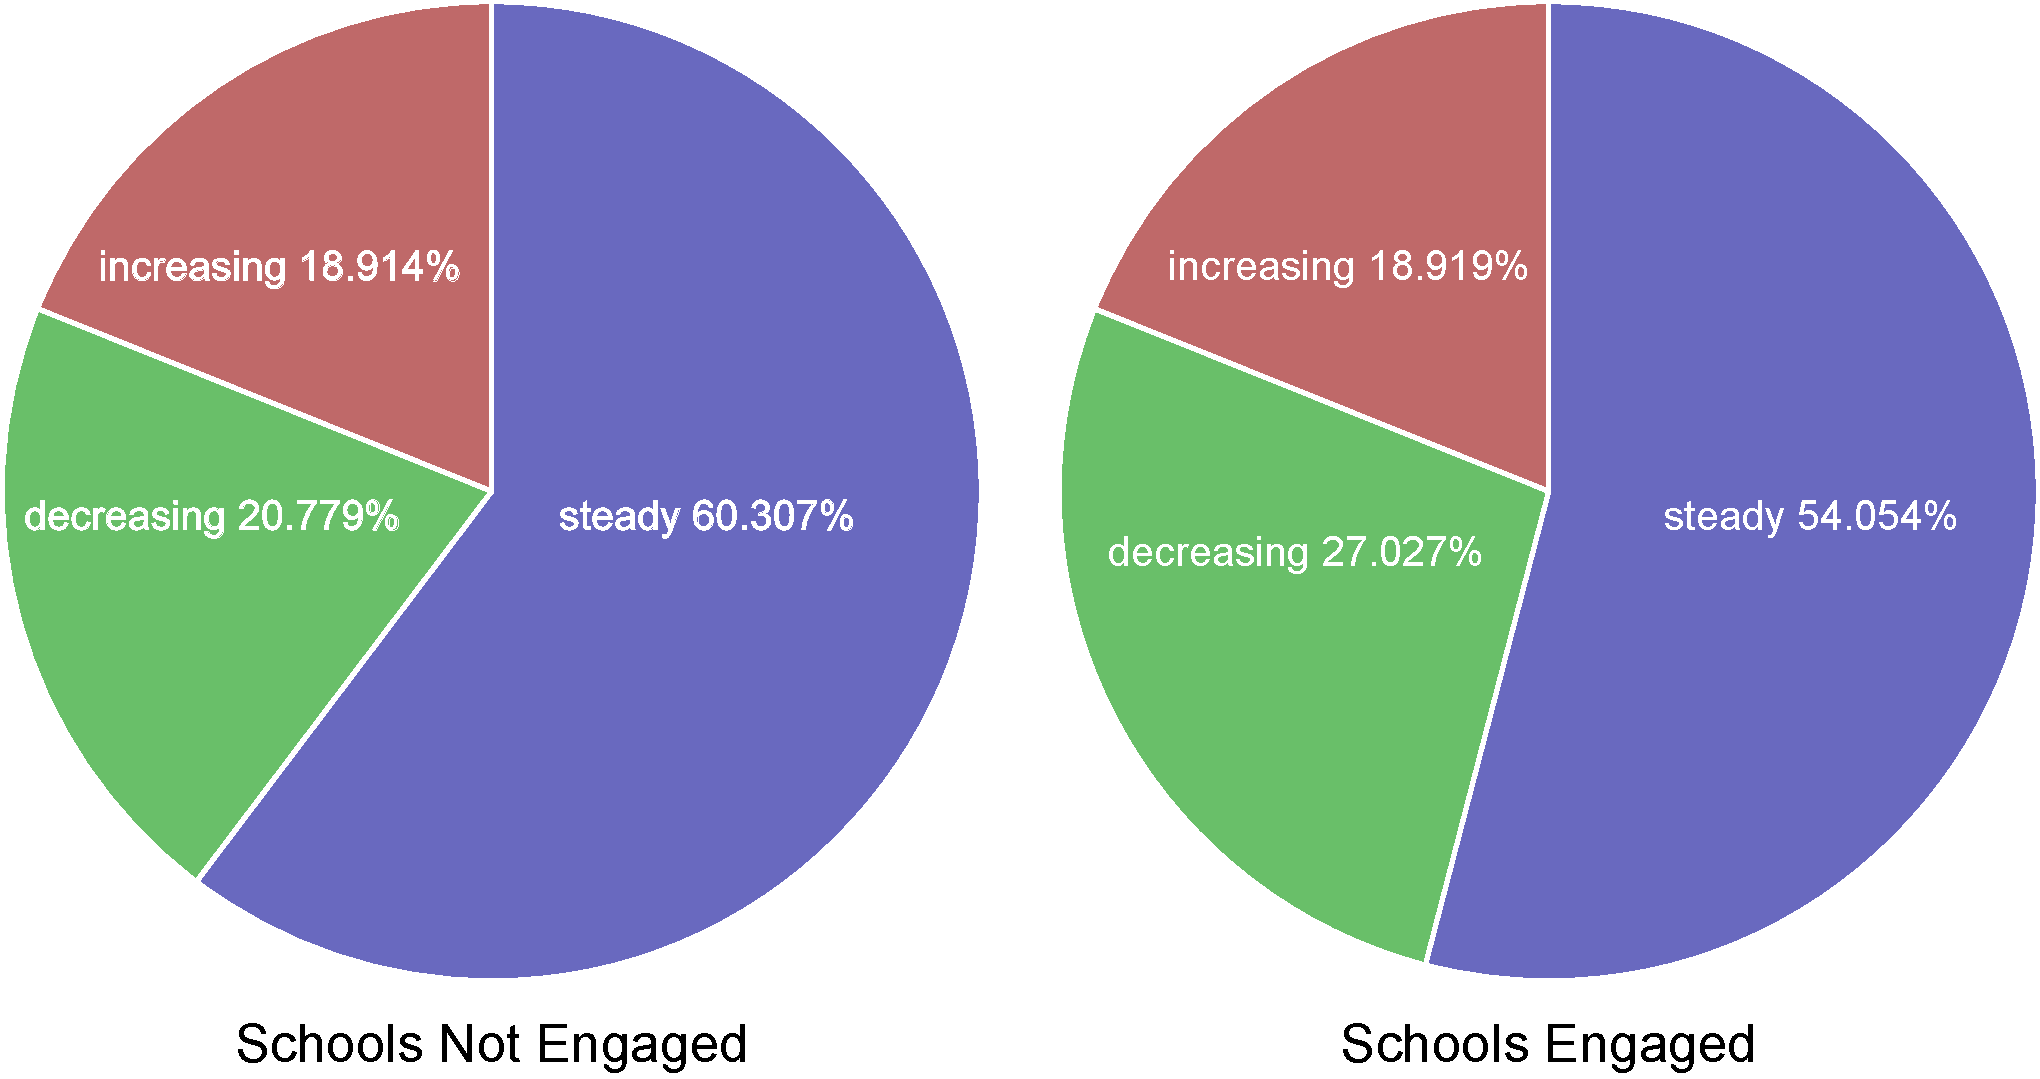
\includegraphics[width=\textwidth]{att_pies}
  \caption[Data:In Place Graphs]{Absence trend graphs made using Data:In Place}
  \label{fig:absence}
\end{figure}

The above marks another milestone towards democratising data science practices by enabling citizens to make sense of and visualise data in context through the use of digital tools. The Using Data:In Place platform participants were able to utilise data to give answers to the hypotheses set by themselves, similar to the professional work done by the author previously (Section \ref{sec:data_prof}). This was also a step closer to removing the researcher from the equation and letting the citizens do it by themselves.
\begin{quote}
    \textit{That's the idea, isn't it? There is no point you sitting here showing me, you doing it for me, because when I go look, I won't have a clue. So I agree, definitely. It will be worth me going away and having a play myself. [...] As I say, I'll try to figure it out. I'll have a play and just give you my feedback and see if I can figure something out. It looks [...] it's coming on. It's definitely getting there. It's exciting, it'll be great. Those graphs that you showed me, very simple stuff, will make some people in the office interested and they'll be happy with what we're doing. I suppose that's the main objective, isn't it? Making people happy?}
\end{quote}
New skills learned by the participant and additional design requirements gathered for the Data:In Place platform marked the conclusion of the second data consultation activity. The participant was happy with the initial results of the investigation; however, discussions about the actual use of them did not get further than `making people in the office happy', indicating the fact that steps were still needed to be taken for the potential use of the data in action.

\subsubsection{Taking Action}
The final part of the data consultation with Charity A (\ref{sec:cs3_design}) concentrated on discussing how the output of data could potentially be used for action. Throughout the process of data consultations, participants identified multiple utilities for using data, such as self knowledge, evidence, measuring and recording behavioural change, getting funds to continue delivering interventions, and a tool for quantifying change.

\begin{quote}
    \textit{We would want to know that personally. So, that stuff we're doing with [anon researcher] is great, but it's' backed up what we knew was happening. If he came back and said, `Look, the kids step counts [physical activity] is going down,' we wouldn't publish that fact, but we would do something about it. So, we would have to be changing intervention.} (SM)
    
    \textit{We've just got to try to do something that evidences what we have done has made a difference to mental wellbeing. For example, we could do a match day campaign. As a result of that, 1,000 people could ring Mind for some support. How do we evidence that's what we did that made people ring Mind and not that just suddenly loads of people decided to ring Mind? We're in the very early stages of looking at all of this. We're going to get another company to help us figure out how we record the behaviour change, basically.} (PO)
    
    \textit{One of the things I'm working on at the moment is going to be an awareness campaign, city-wide, through match days and our social media, amongst other things, trying to improve health and wellbeing. We want to be able to prove that what we've done has made a difference.} (PO)
    
    \textit{That's where our health and wellbeing department is at the moment. We've got that aspect; we've also got the bit that I'm doing in terms of the targeted mental health intervention. If we're trying to relate that to data and place, for me, I know that I'm going to have a 12-week programme in which they'll be sessions which try to improve the mental and physical wellbeing of the guys that take part. Looking at the long-term behaviour change and the long-term measures of those that I take at the beginning, over 12 months would be great.} (OO)
\end{quote}

Those aspirations for data were guiding the participants in the hypothesis setting and investigation parts of the consultation, aiming to come up with outputs that serve those needs. Participants were focusing on the two main aims for the data output: (1) official documents and (2) presentations.
\begin{quote}
    \textit{If we were reporting... say, if we had funding, and we were reporting back to the stakeholders or the people that funded us, then a graph would be a good visual tool to use. In terms of writing a funding bid, it's the facts that we would need, percentages or official figures.} (SM)

    \textit{We want the facts and figures for [...] yes, official funding documents or reports to stakeholders. Then we're going to settle on easily-digestible... What are they called?. Infographics using the [Anon Sports] club as a metaphor, I suppose.} (OO)
\end{quote}
When presenting the data to people outside the organisation, participants felt that the data outputs needed to be converted into something that represented their identity, which also came up in the first part of the data consultation. These custom infographics could potentially be used to reach different audiences through a multiplicity of channels.

\begin{quote}
    \textit{I think for your average-joe consumer, it's plain, simple facts. As an example, we've got an event on the 22nd of March when we're inviting a variety of schools that we've worked with and schools that we've never worked with [...]. This is going to be a room full of teachers who are in charge of budgets. We want to sell, to them, our product. If, at some point, we can say, `Up on the screen now, you can see that these are the schools that we haven't been in, their attendance, behaviour, and homework. These are the schools that we have been in, their attendance, behaviour, and homework. As you can see, there is a significant change between those two.' When we go into a school, we now know that these things improve. That would be a visual thing. It wouldn't be, `Let me read from a paragraph and give you loads of statistics and loads of numbers.' People wouldn't get that.} (OO)

    \textit{They [organisation marketing officers] might go to that school, knock on the schools door if they've never been in before, and now might take with them this infographic. They might go, `Look, this is a simple way of us showing the impact that we've got, the impact that we've done in the region. The schools that we've worked in with [Anon Programme] have beaten the away team, the team that hasn't had [Anon Programme].' It would probably be the same infographic as what was used in the presentation held at the stadium. That would be taken and put onto some sort of booklet or brochure or easy-digestible material that they can take to schools. That's probably our two ways in which we sell, I suppose.} (OO)

    \textit{Infographics are great because they're also shareable. If you put that on social media, people are more likely to go, `Oh, I'll share this.' Then, it just gets… It's more awareness of the foundation as a whole, isn't it, rather than it just being just a graph.} (PM)
\end{quote}

However, making these customed infographics was something that could not have been achieved by the participants themselves, even when using the Data:In Place platform; in this sense, they would have needed support of a data visualisation professional. Throughout the consolidation process, that person was the author of this thesis, who assumed the role of the data professional. Going forward, there was a need to find new ways of providing that expertise to people that does not involve support from the researcher.
\begin{quote}
   \textit{I think what you're saying is you know the answers, you know what the data are, you know all those different things and know the questions with those answers, and it's creating those pathways which I get that [...].} (SM)
    
    \textit{There needs to be somebody who's not you, who's got your skill set but is able to do that. I suppose you probably know more than we would whether or not there are people out there that would be incentivised enough to answer the questions and challenges.} (OO)
\end{quote}
Participants here were starting to think about how these connections between data professionals and issue owners could be created and mediated through digital systems.
\begin{quote}
    \textit{It would almost be like a message board that challenges one to start with. [...] I guess a lot of the stuff we always ask is often the same, so it will just be like first run through and asking for data and it's usually general.} (SM)
\end{quote}
This was significant because it would open up new opportunities for potentially expanding the skills network of Charity A and reaching out to external parties. Although this was promising, the participants saw multiple barriers due to the temporalities of these `data challenges' and ways to incentivise individuals to take them up.

\begin{quote}
    \textit{I mean, we can post as many challenges as we want in terms of we want to know something in a certain area. A lot of the time, it's last minute as well. It'll be like, right, we need to know who's doing what in here within the next two weeks. So say, for example, we post that on this system here who's going to pick that up. Why would they pick it up? Is it because they want to be socially doing more things for the society and things? You'd probably know more than me because you're sat in that position and representing that individual, whereas I personally, when I go home from work, I don't want to go back to work. So whether or not that guy picks it up on the other end and whether or not he can turn that around within two weeks will probably be the task.} (OO)
\end{quote}
Additional barriers that surfaced included unwanted competition, safe ways of sharing data and establishing trust and credibility between issue owners and challenge takers.

\begin{quote}
    \textit{I suppose there might be a bit in there in terms of, say, you've got a chat board or a chat room or whatever it is on here, everybody can see that [the organisation] has just asked, does anybody know what the crime rate is like in the west end of Newcastle? Other people might go, `Why are they asking that?' Then, that could suddenly increase competition for certain bids as well.} (OO)
    
    \textit{I suppose it's what you were saying before -- how do we then trust that person, how do we know who that person is in a way. So how is that person verified through the system or through a different web because it could theoretically be, it could be then walking down the hill.} (SM)
    
    \textit{That could be a 12-year-old kid in his room, and he's just got computer (OO). Get some data and just likes chucking it all over the internet somewhere, which hopefully it wouldn't be, but you never know really, do you?} (SM)
\end{quote}
Indeed, it was important to establish trust between both parties to work together exploring and using data. It was not only an issue of asserting confidence in challenge creators but also of making sure that questions and challenges posted were coming from valid sources.
\begin{quote}
    \textit{[...] if I'm asking questions on here, `Hey, does anybody know how many overweight and obese men there are in the north east?' then that might make somebody go, `Well, hang on a minute, why is he asking that?' If it was just at random, I think if nobody's got their name attached to it, people would be more willing to... [pick it up]} (OO)
\end{quote}
The participant here went on to discuss the ways challenge takers could be verified on the web and trusted by challenge creators:
\begin{quote}
    \textit{Bio almost, with even links to other stuff that you've done in the past.} (SM)
    
    \textit{I'm going to trust our Eddie, who's got x, y and z or hundreds of publications on data science more than I am Jimmy, who's 12 years old.} (OO)
    
    \textit{And our Ed works at Newcastle University part of Open Lab at Newcastle University as opposed to Jimmy, who's 12.} (SM)
\end{quote}
Data science professionals spend years honing their craft, undertaking a range of projects to obtain the skills needed to work with data and produce valuable outputs from it. Participants saw an opportunity here to potentially give learners a chance to take up projects to improve their skills and solve real-life problems.
\begin{quote}
    \textit{I suppose your future pool of people could be undergraduates or post-graduates who you want to build a portfolio as a data scientist.} (OO)

   \textit{[A] real-life programme and challenge for a company while studying, that's probably one of the issue for students.} (SM)
\end{quote}
One of the ideas participants proposed was also to build an ecosystem around data challenges that would enable a community of data scientists to grow and sustain the service.
\begin{quote}
    \textit{I suppose if you want starting off small with your smaller community of data scientists in order for them to want to do this, incentivise them with a potential stake in the company or whatever it is or in your page or a stake in the interest of it as opposed to suddenly become they're your panel members and your decision makers of who is awarded certain statuses as future data scientists.} (OO)
\end{quote}

The data consultations guided people through the complete process of data use and provided an in-depth first look into the cognitive processes that people go through in order to find, access, make sense of and use data in action. The findings presented here enabled further understanding of the model of CDI in terms of how people posit questions for data and the ways data can be accessed by people, transformed into a useful form and leveraged for actionable results. The data consultations provided new design considerations for both the methods of inquiry and the digital tools that would aid and mediate them, both of which are crucially important for the \textit{social facilitation} (Chapter \ref{chap:cdi}) of the effective use of data by communities. Lessons learned from the data consultations were applied in the second engagement activity with the local community.

\subsection{Community Action Day}
\label{subs:community_action}
Building on the findings of data consultations, a workshop around making the use of data in community action effective was undertaken. This section presents the findings from that community workshop, where a set of methods and digital tools were trialled in order to explore their usefulness in guiding people through the process of using data in community action. The reporting on this phase follows the process described in the Study Design (Section \ref{sec:cs3_design}) and illustrated in Figure \ref{fig:cdi_phases}. Because of the nature of the workshop setting and having a lot of cross talk in the transcriptions, the community is represented as a united voice and quotes are presented without pseudo identities. Distinctions are made, however, between the two groups formed in the workshop.

\subsubsection{Issue Mapping}
Issue mapping through the use of CC provided people an open space to bring any issue to the table. Participants were asked to use prompt cards (Figure \ref{fig:ccv2_cards}) to provide more information about issues flagged in previous sessions (Chapter \ref{sec:datainplace}) or to add completely new issues to the map. Although people had the freedom to do so, throughout the longitudinal engagement with the local community, a particular set of issues kept coming up and being identified by the community, which were linked to things like a lack of facilities for kids and green spaces that people in the neighbourhood could enjoy. Participants turned back to discussing these issues, some of which had also been marked in a previous Community Action Day where CC was used. The utility of tools such as Data:In Place or Ambit (the technology behind CC) was not only to document these processes for further use, but also to provide anchoring of these issues by situating them.

Issues that people were identifying were mainly observations about different places in the community that they wanted something done about. As mentioned before, many of the issues were linked to underused fields or green areas that had been neglected and were in need of maintenance:
\begin{quote}
    \textit{It's on your left side and down the road, isn't it? 
	Where Ronsons was, and then they got all the derelict ground.}
\end{quote}
\begin{quote}
    \textit{You got a lot of area out there on [Anon] Road, haven't you, that's just like lying derelict.}
\end{quote}	

Participants felt that these spaces could be utilised better, for example, by providing activities for young people who did not have any facilities:
\begin{quote}
    \textit{Nothing, nothing. Absolutely nothing. Sometimes, it does get used for kids drinking on the field, hiding in the bushes, [and] so forth. So, I think a lot more could be done with that area there. They could have a lot more for the kids to play on there.}
\end{quote}

Although participants were noticing these issues in the community, they felt that others, e.g. the local government, needed to do something about it. There were also ideas of establishing new housing and businesses or allotments on those `no man's lands'; however, participants shifted the actions back to the local council: 
\begin{quote}
    \textit{I mean, the council could put into plan a cheaper rent for people to start their own businesses, or anything like that.}
\end{quote}
\begin{quote}
    \textit{Isn't that because the council have a long list of people who would like an allotment and the council are so slow at informing the people when the allotments become available.}
\end{quote}

Using the prompt cards and taking turns flagging and discussing issues, both groups ended up with a set of marked issues on the map. The activity was set up in a way that people could express support or agreement with others through the 'second that' prompt cards, helping to filter out issues that were most important to people and preparing for the next activity of prioritisation.

\subsubsection{Issue Focus}
To move onto exploring an issue, participants had to prioritise flagged issues by discussing them amongst each other and listening back to recordings of other people's opinions before finally deciding on which issue was the most important to them. The mechanics of the CC already helped bring some of the issues forward that multiple people felt important for improving in the community.

As mentioned before, an example of `rock climbing` (chosen by the thesis author) was provided to guide participants through the next steps of the process and the question formulation. However, having already gone around the map in the first activity and identifying issues provided the participants with a better, more anchored focus. One group took ownership of an issue regarding the lack of facilities for children -- \textit{`[We] want to focus on [Anon] Way, because there is nothing there for the kids'} -- while another group focused on green areas and wanted to \textit{`repurpose [Anon] View playing fields'}, where half of it was used by a local football club. Once the focus was agreed, each group used Data:In Place platform's mapping function to document their focus and make it visible to the other group. This provided each group with an issue to focus on and a location to anchor it to before moving on to exploring it further through questions.

\subsubsection{Question Asking}
At this point, participants had identified and flagged issues, listened to other people's opinions about them (both live and recorded), discussed them within the group, and chosen a focus for their investigation. They had then to use that focus and apply it within the QFT that was modified for (Section \ref{sub:qft_action}).

When people started asking questions about their issue, they were not constrained only to what they wanted to see in those places or \textit{`what it is used for currently'}. Instead, people had a more exploratory attitude, promoting curiosity and discovery, coming up with questions like:
\begin{quote}
   \textit{What would we like to see there?}
   
    \textit{How much would it cost? [and] Where would the money come from?}
    
    \textit{I wonder if there are any people who have already seen the places. What have you seen in the parks that you think we'd love to have?}
    
    \textit{Would a sports day be -- I don't want to say popular -- community sports day be something you'd value?}
    
    \textit{Also, how much would it cost to maintain? It might be like an ongoing thing.}
\end{quote}

Asking questions about the issue also shifted the focus from `what the council can do' to `what the people themselves or the community can do':
\begin{quote}
       \textit{[The] first one would be what can \textbf{we} do with a bit of grass?}
       
       \textit{How would \textbf{we} go about changing it? The likes of who would \textbf{we} have to see?}
       
       \textit{We can only try. If \textbf{we} get the funding on it.}
\end{quote}

When people worked on their questions according to the QFT method (for example changing the openness of them), they also reflected on their own role as community leaders or spokespeople for the community, perhaps using the same questions to give voice to the wider community and get more opinions forward:
\begin{quote}
   \textit{Actually, between them two and these two [questions], what I've changed is you're not giving people the option on what they would want there as in what- what was it then we changed, number four? We're talking about the green area behind a specific thing, and to me it would be a park, but on my first question, what would you like to see there? Now that gives everybody and anybody a chance to say what I would like -- a bike park, skate park, this park, that park. My next question is would a park benefit your children?}
    
    \textit{So, I probably shouldn't even use the word `park', because that limits it a bit, doesn't it?}
    
    \textit{How do we go about changing from what it is now to what we want it to be? Or what the community wants it to be? It's not what we want it to be, is it?}
\end{quote}

Additionally, questions sparked discussion around the way participants could figure out the needs of the wider community, make them visible to everyone and get the community involved in delivering those changes for the neighbourhood. These points were the main considerations when prioritising questions for investigation and challenge creation for both groups:
\begin{quote}
    \textit{So, our priority questions were: What are the options for the use of the space? Quite broad. What is lacking in terms of the existing local provision, facilities? Then, what is the space already used for?}
\end{quote}
\begin{quote}
    \textit{Our three questions were, because we would like to see more things on there for kids, so our three questions were: How do we get the community involved and maintain their involvement? Because if not everybody wants it, then it is not plausible really, is it? It's got to be everyone on board. Our second question was: How do we go about changing the space to make it what the community want to see? Our third question was: who would fund this?}
\end{quote}
Applying QFT on the issue focus set the groups up to have concrete questions at the end of the process, which set the tone for the challenge creation activity.

\subsubsection{Challenge Creation}
Challenge creation aimed at breaking down each question using the prompts provided with the worksheets (Appendix \ref{app:community-action}). Because both groups were looking at green areas, it was important for people to figure out who owns those lands first. People always assumed that land was owned by the council, but nobody knew that for certain. This was a clear challenge in terms of \textit{data access} to obtain the information of land ownership.
\begin{quote}
    \textit{I always thought, `Who owns the deeds of that land?' You know, because obviously I think they should be...[owned by council]. Then, of course, the football team comes into it but owns that last 50 percent of the field or whatever is left of it. Is it [the] council or is it private land?}
    
    \textit{So, local knowledge, council. Presumably, do the football club own their little patch?}
    
    \textit{Yes, it's finding out the ownership, yes? So, what I was saying about the idea of finding out what the options are for how to use it.}
\end{quote}

Another challenge identified by both groups was to figure out the current uses of those two spaces: \textit{`I wonder if the idea of the, what's the space already used for? That's quite a key question, isn't it, really?'}. People had some ideas of the uses based on the observations of \textit{`there is walking access, [...] there are a lot of dog owners that use it [the paths on fields]'} and \textit{`there is a metal seat there, and there are metal goalposts, and a hoop [...] kids do use that [...], but sometimes it is full of glass and that'}. Additionally when asked if there was any data about it, participants said that there was nothing they were `aware of'.

In terms of data challenges, this was a challenge for \textit{data production}. This could have been done by observation or by compiling all the local knowledge of the workshop participants, but people thought this could be a good opportunity to collect data from the wider community -- people's current uses of the fields and their ideas for the future. This was a challenge that resulted in suggestions for immediate actions that people themselves could take it rather proposing it to someone externally.
\begin{quote}
    \textit{Right. To collect the data, or what people think, we would do a questionnaire. We could go door knocking in the local area. Yes [to figure out what people think], and in general if people would be interested and that.}
    
    \textit{Actually, I think you would have to put it into a different thingy. Not what would you want to see there? Because you could have one person wanting that, that and that. If you said, `Would you be interested in a park being put on?' [then] it would be a closed question, as in yes or no. Then your piece of paper would just be two. Or it could be three. You might have someone who says, `Maybe.' (Laughter) Then you would only have two, and then it's pros and cons, isn't it? Yes and no.}
    
    \textit{Do more people want a park than not?}
    
    \textit{So, I think the collecting stuff ourselves thing, that's going to be what people would want to see it used for, isn't it, and what they're already doing. So, there is potential there for collecting data from existing usage and that, potentially.}
\end{quote}

This would also extend to not only collecting the current uses of the fields but also getting people involved in thinking about what can be done with the spaces.
\begin{quote}
    \textit{So, as in, what do they know that's elsewhere that they'd like to have on their doorstep [...]}
 
    \textit{I know this sounds like Eden, you know that big project down in Cornwall? A local communities thing called the Eden Communities that helps local communities to repurpose green spaces and that sort of thing or to organise themselves.}
\end{quote}

This also sparked conversations around compiling data of things people do in their free time and figuring what the current available pastime facilities are in the area or neighbouring areas, creating multiple challenges for data in terms of \textit{data access} and \textit{data production}. 
\begin{quote}
    \textit{We could do with all this, knowing what the council provisions [...and] a little bit of just local knowledge that we could use there.}
    
   \textit{Yes, so actually even knowing that exists there is going to be useful, for just knowing what the options might be for knowing about the other facilities [...]}

    \textit{There was one over the, I think it was Station Road in Newcastle. If you come off the [crossroad], you go down over the bank, there's actually a massive park which has everything, obviously swings for kids and I think one looks like a full-sized basketball -- a tennis court, whatever, but they have full-sized court there, which is -- but I don't know if it's still there or not, but it looks like there's a park for kids, swings [...]}
    
    \textit{I can't remember what information is in the census because, you know, you can get the anonymised data from the census from 2011, whether that would have anything about what the pastimes... I don't know if that's in there. You don't happen to know?}
\end{quote}

Data challenges not only focused on the first part of getting the data (i.e. data access and production) but also got the participants thinking about challenges that would follow once the data was obtained or collected. These challenges were linked to \textit{data visualisations} that prompted people to think about how they could turn that data into something useful. Participants thought that it would be best to present that data back to the community to gather support and get feedback on ideas. 
\begin{quote}
    \textit{I think you could put it into a leaflet. We could put one through the doors or if you go on the computer, then that's all that data on there.}
    
    \textit{With the computer or just talk, have a chat sort of thing.}
\end{quote}

This would potentially include data collected from the community using questionnaires, which are process as \textit{`[...] information in simple numbers, or graphs`}, \textit{`then you would probably put them into categories. Would people want it as this, this or this'} and merged with data from official statistics \textit{`to give a simple answer everyone can understand'}.
\begin{quote}
    \textit{The questions would... What would you like to see on the field? What would you like to see the field used for, blah, blah, blah? When the questions are all done, stacked up.}
    
   \textit{So, from any data that we would collect from door knocking or talking to people, or whatever, that could be presented in a... Fifty people said, wouldn't it be fab if we had a kids' playpark. A hundred people wanted a...' So, there could be some graphical representation of [statistics].}
    
	\textit{Could we also put in something there about the census pastime stuff as well? So, you know, we've got 300 people from the [X place], who love to cycle.}
\end{quote}
However, not only were people interested in representing people numbers and official statistics, they also wanted to seek feedback from people and start contesting these numbers:
\begin{quote}
    \textit{If we stuck in a bike park, it's a bit of -- they don't quite [add up]. So, just [If you point your finger with that sort of thing there], then there is a load of cycle tracks, but if that's the place you mean?}
\end{quote}

Participants were interested in presenting data about the spaces -- what exists, current uses and potential ideas -- in a way that was more interactive and representing the community identity.
\begin{quote}
    \textit{Yes, I guess the visual representation of the space, we're just using a map of the space and saying, `That's already the football thing. That's already this. This is the space we're talking about' which represents the landownership bit.}
    
    \textit{So, if you have an idea of what the council provision of their facilities have already got somewhere else, there's potential, isn't there, to stick some pictures in of the fact that they've got a skate park here. The likelihood is we're not going to put something there, but just to say, `That's there. There's a bowling green there.' There's whatever.}
    
   \textit{I guess you can, sort of, mark bits out, so people can go, `Could this be this? Could it be that? Could it be that?' I wonder as well, if you were going to do a leaflet for the [Blue Sky Way's] bit, then there's potential to just say, `Oh, this place in Sheffield has this and green space like this place. There has that...'}
\end{quote}

Perhaps the biggest challenge people identified was how to fund the development of these spaces and where they would start looking for such funds.
\begin{quote}
    \textit{Well, it's got to be the big one, isn't it? Where would the funding come from? Where would the money come from?}
    
    \textit{But we could put it to the council, but then you could also put it out to... Oh, I don't know. I would probably ask where could I go to find funding for it?}
    
    \textit{Yes, so I guess presumably different funding bodies will have very specific things they want to do and stuff.}
\end{quote}

Participants were not only thinking about how they could convince the local government to fund these changes, but perhaps there were alternative ways of funding it, looking at how they could collaborate with other organisations in the community and even outside of it
\begin{quote}
    \textit{Maybe get some businesses on board. There are local businesses around here. There are B\&Qs. There is GTF. Actually, there are also another two community centres. There is the [Anon Organisation] and the thingy, so maybe they could help.}
    
    \textit{Oh, yes. Presumably, there might be someone that can say, `Yes, okay, we've got a specific pot of money, and we would build a kids' playpark,' or, `We've got a specific pot of money that'll do this or that.' That might influence what you end up doing.}
\end{quote}

For the last activity, participants were brainstorming actions they could take with the data. Their initial idea was to compile all the data and then seek feedback from the community to build support:
\begin{quote}
    \textit{Yes, I mean, so in terms of making the information actionable, are we going to say to people from this leaflet, `Give us a tick to say, 'Yes, we'll want to do that,' or a cross to say, 'No, I don't want to do that.'}
    
    \textit{Yes, or do we say, `Just come along to the meeting and we'll talk about it at a meeting,' and present a much more concrete ideas about things.}
    
    \textit{Getting all the community together to brainstorm something like that. I know you can't keep everybody happy.}
    
    \textit{I guess, in this exercise, we're assuming that if we're doing this, there's a certain level of buy-in, we're happy, as people, doing this to galvanise a bit of... You know, if we're talking about doing something with here, we're happy to lead a bit on saying, `Come and get behind this, we're going to do something with it.'}
\end{quote}
and then taking that information to the local government:
\begin{quote}
    \textit{You would have to get a meeting with the council [...]. We would have to contact the council, wouldn't we?
    You would take your findings from that to your council.}

    \textit{If everybody agrees, then you go to [the] council and just say, `This is what we'd like to happen.'}

    \textit{[saying to the council] `This is what the community wants. We have done that door-to-door. We have done whatever is needed'}

    \textit{We sort of show them the data, do we, to say that this has got community backing?}
    
    \textit{Yes. Ask the council if there is anything they can do, even if it's half.}
\end{quote}

\begin{figure}[htb!]
\centering
 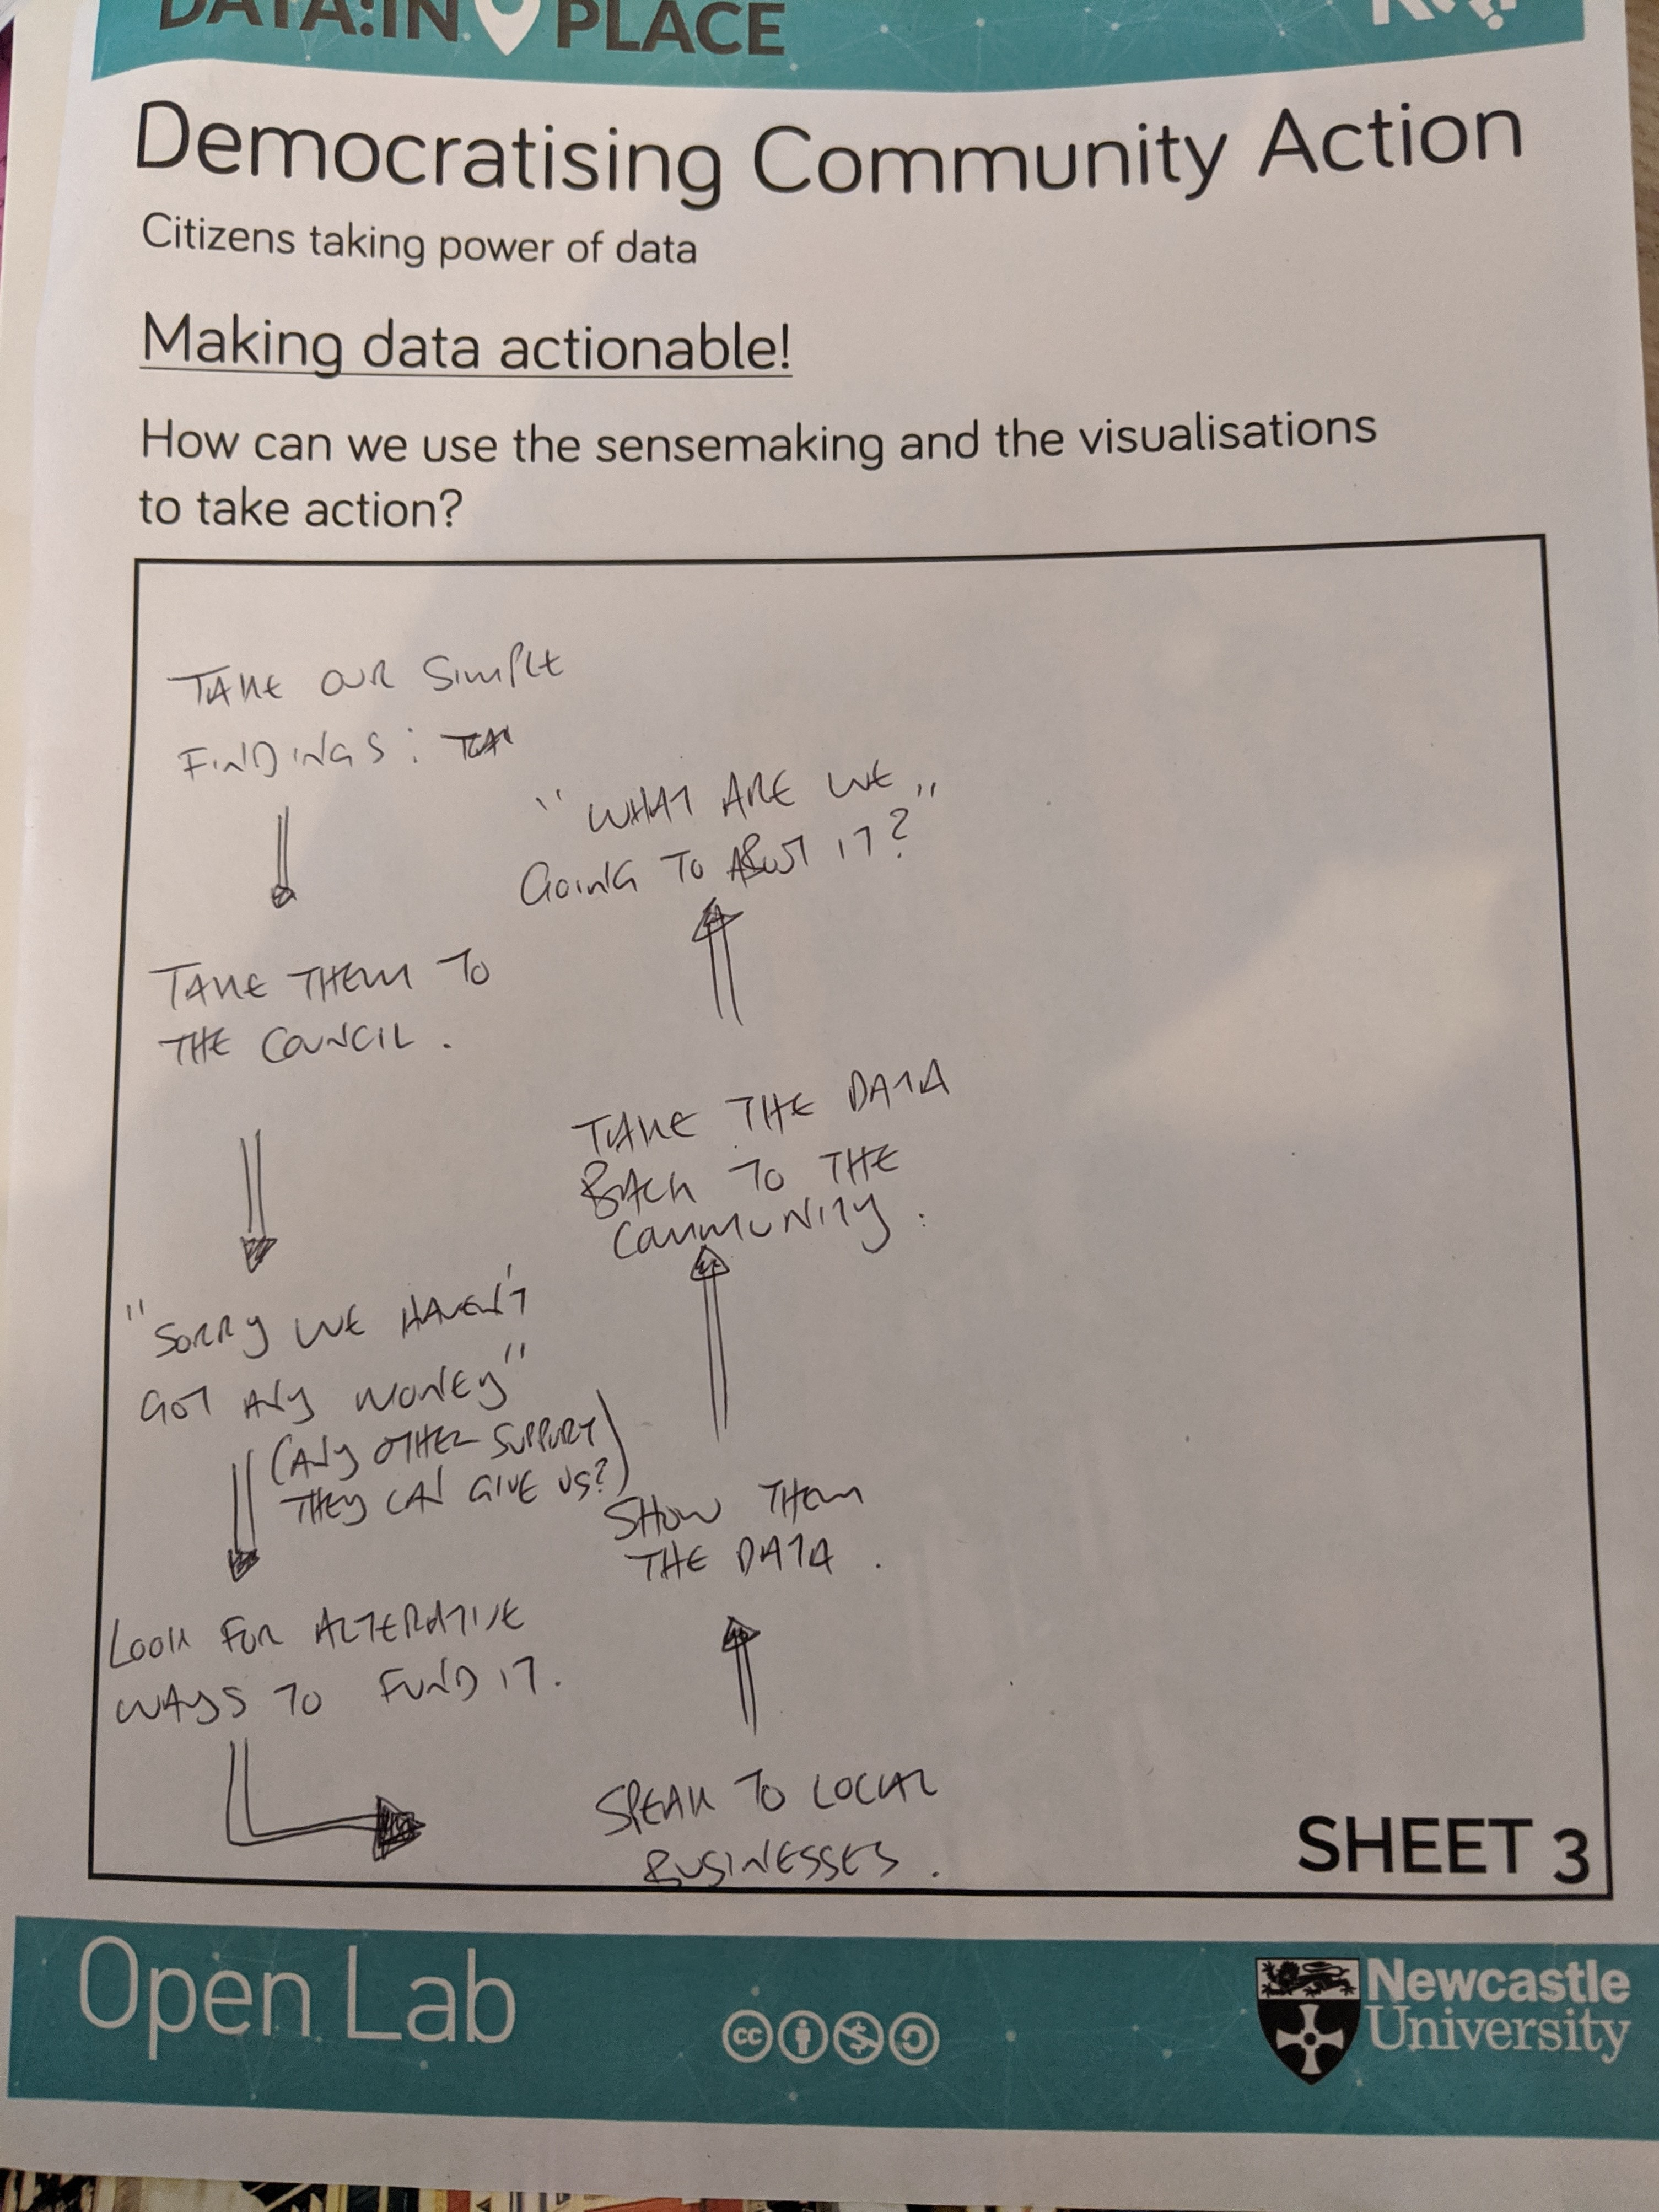
\includegraphics[scale=0.1]{action_plan}
  \caption[Community Action Plan]{Screenshot of proposed steps for community action}
  \label{fig:action_plan}
\end{figure}

Participants were not really convinced that the council could do anything and they would probably respond with \text{`[...] It's gone past our budget for this year, sorry. (Laughter) That's what they'll say.'} However people started to shift into the mindset that perhaps the council did not have to do it all and there were ways to do it together with the community.
\begin{quote}
    \textit{Yes, but maybe it is not all about them doing everything. It's making them aware that the community are willing to help as well.}
    
    \textit{So, I guess, almost then using that as the start of trying to gather people together, affirmation of it, so people say, `Yes, we would do that,' or, `Yes, I want to do that, and I'm also willing to put the time and effort into making it happen.'}
    
    \textit{Are you [member of community] painting? Are you digging holes? Whatever it may take.}
\end{quote}
Here, the participants used the challenge creation activity to think about not only what others could do to make things happen for them, but also to look at what actions they could take themselves, finding skills within the community and also using the Data:In Place platform to post data challenges to get access to professional expertise externally. Figure \ref{fig:action_plan} illustrates the proposed action plan of one group. Furthermore, statements such as \textit{`it would have to be a community project'} represented the realisation that it has to be a collective effort of the community, where data could potentially be used to foster dialogue between different stakeholders and bring the community together to take action.

\section{Discussion}
The dual approach for CDI facilitated the process of discovering ways that data could be made actionable. A process of inquiry and asking the right questions enabled people to form a better understanding of what data they might need and plan out steps for actionable results. The findings contest the ways that data is currently projected \textit{to} and \textit{about} local communities, in addition to opening up new possibilities for better knowledge making and more meaningful \textit{CDIs} to take place. The following sections discuss the findings of the case study, reflecting back on the questions and aims of the case study (Section \ref{sec:cs3_design}) as well as the model of CDI in practice.

\subsection{The Power of the Right Questions}
Many scholars in HCI have made a strong case for the importance of curiosity, discovery and inquiry in the participatory design process of exploring issues \citep{marres_issues_2007,moor_beyond_2007,disalvo_neighborhood_2008,dantec_infrastructuring_2013,balestrini_beyond_2014,balaam_feedfinder:_2015}. However, there is an inherent difference between observation and investigation of matters of concerns. The case studies in this thesis have shown that flagging issues is useful for providing new observations about things people are concerned about. These are useful in many regards, especially when mediated through digital tools, providing a way for people to express their concerns, resulting in a new and interesting dataset. This type of crowdsourcing of data is common in large-scale participation projects \citep{dantec_data-based_2014,liu_crisis_2014,thompson_crowd-sourced_2016}. Archived collections of citizens' opinions serve as interesting datasets for researchers working at the intersection of qualitative and quantitative data. There is a risk, however, that the mode of citizen participation is often abstracted to pins on the map (see literature review Chapter \ref{chap:literature} for different modes of participation) and not engaging with citizens to become the active users of data.

Unfortunately, in a lot of cases (also illustrated through the case studies in this thesis), these observations do not necessarily always follow any actions. The reasons for this may be linked to factors such as a lack of understanding of the issue, complexities surrounding decision-making processes that bring upon or instrument change, and a lack of community support or perhaps a lack of evidence. Although data might be `out there' or there are ways to generate it (for example, using the toolkit described in Chapter \ref{chap:sensemystreet}), people often feel powerless and suffer from an inability to take action. Early in the process of defining issues, people were pointing out places (using the Data:In Place platform and functionalities of Ambit) in the community that they thought someone needed to do something about, for example, places where youth engage in anti-social behaviour, rundown housing estates or neglected derelict grounds. The pressure was put on the local council to `sort these places out', and people assumed that they cannot do anything about these issues themselves. However, in many cases, the community problem-solving activities needed issues to be better articulated and dissected by community members.

Introducing QFT into the process of inquiry by choosing to focus on something particular and starting to ask questions about issues opened up alternative views and possibilities around taking action, whether it was connected to bringing the issue to light in the eyes of the wider community or even `rolling up the sleeves' to put in the work themselves. This also extended to a better understanding of what data (and other resources), capacities, and infrastructures are needed and what actions need to follow. Furthermore, having concrete questions helped people to understand the roles that needed to be filled and the constraints they were working against in a given context, all promoting actions that extended from getting and understanding the data to what was equally important: How that data became interpreted and presented to others, thus shifting the end goal from \textit{getting access} to the data to \textit{making data actionable}. This also challenges the ways citizen participation through data should be perceived, recognising broader interactions and the extent of how data could be used by communities.

\subsection{Holistic Approach to CI}
The practical approach for the CDI was put forward though the dual approach method described in Section \ref{sec:dual_cdi} in order to better understand how CDI works in practice. \citet{hakken_social_2003} points out that the main aim of informatics, as an engineering discipline, is to design AITs that work. This often lends itself to building abstractions that are distanced from the social and/or contextual dimensions important to knowledge-making processes. In the context of CDI (Chapter \ref{chap:cdi}), these are the key elements of the model that are bounded by the factors that influence these elements and also become the domains of change. Using an approach that facilitates the functionalities of digital tools and data enables not only an understanding of these dimension but also helps accommodate the use of AIT to already existing social contexts. In the case of the participants in the study, these were linked to the historical relationships between residents and decision-makers or current practices of the local community organisations. These contexts became part of the process of inquiry, helping bring issues to public attention and making people reflect on their own practices by thinking of the ways things have been done before and how they could be done in the future. Digital tools that accompanied these processes acted both as enablers and historians of sensemaking by creating digital trails of people's interactions. Studies in HCI and participatory design have demonstrated the benefits of capturing different voices and situated understandings, enabling a multiplicity of narratives and social interactions to come to the surface \citep{manuel_participatory_2017,rainey_gabber:_2019,bartindale_our_2019}. In many ways, the processes engaged in data consultations and Community Action Day served as means to bring attention to relevant contexts so as to interpret and make use of abstract open datasets available through Data:In Place. Although Data:In Place and its functionalities were generically built to enable better access to and exploration of open datasets, their appropriation was highly related to the communities using them and their identities. This related to the datasets needed and was relevant to not only the issues people were faced with but also the way data had to be represented to include the visual identity as social context. For Charity A, these were things that associated them with the local sports team, while for the neighbourhood planning group, these were things that represented community identity, making data relatable to the local residents. However, this context needed to be brought out by people and intertwined with the data and its formal representations.

As information and knowledge are situated and constrained by interpretations \citep{suchman_plans_1985,suchman_human-machine_2007}, this makes it difficult to use IS to convey that needed context. According to \citet{devlin_infosense:_2001}, however, it is impossible to embed context into information -- it should be extracted from information, and the most we can do is to provide an indication of what the context might be. This formal abstraction has been criticised by people in SI because it is contradictory to the social understanding of information and knowledge \citep{hakken_social_2003}. However, both sides agree that in order to recover knowledge from representations of information, a social interaction is needed. While face-to-face interactions are the preferred way of knowledge networking, alternative approaches such as embedding the context in representations of AITs and supporting knowledge-making processes around them should be considered.

With regard to social readings, \citet{hakken_social_2003} provides an understanding of why such approaches are more likely to have the desired outcomes. In this sense, he states that \textit{`different understandings of functionality in software would provide a better key to developing a more satisfactory approach to the problem of mediating knowledge networking via AIT'}, and the \textit{`goal should be to find AIT-mediated forms of knowledge representation that functionally equal the sociality of existing knowledge networking'} \citep[p. 156]{hakken_social_2003}, thus making the main goal of AIT system to implement ways that enable to encode as much context into formal representation of data as possible in order to support knowledge creation and action. He calls these \textit{applied social informatics of knowledge (ASIK)} systems, which combine ideas from User Participation in Systems Development or Participatory Design (PD) \citep{dahlbom_computers_1993} and CSCW \citep{winograd_understanding_1986}, acknowledging that most of the work take place in groups. 

Drawing on \citet{hakken_social_2003} and others in PD and CSCW, an instance (or perhaps a manifestation of the author's experiences and PD process) ASIK was also designed and built in this particular case study following a longitudinal engagement with stakeholders from the local community. Moving away from purely information engineering approaches to social and community informatics, and through the use of CDI, enabled a more holistic approach to how data is accessed, interpreted and made useful by communities to be taken. The findings suggest that the dual approach for CDI, using Data:In Place with QFT and Challenge Creation, helped facilitate the process of contextualising data and provided conditions for actionable knowledge to be created. The process of inquiry often revealed that the required data was not as complicated as initially perceived, and through contextualising, it could be presented by means of simple visualisations that people could do themselves or by using the Data:In Place platform. Additionally, the future directions of the platform may consider ways that knowledge networking can be expanded by brokering the communications between different stakeholders, both professional and non-professional.

\subsection{CDI and Collaboration}
The findings from this case study (and from Case Studies II and II) highlight that when it comes to data science skills, there is still a need for expert professionals to provide guidance or lend their skills. Even if some processes can be mediated by intelligent systems -- such as was illustrated in the case study when local Charity A was using the Data:In Place platform to access school performance data and correlate it with their engagement data to produce visualisations Ð data often still has to be found, processed, mediated and/or put into these systems. Without a strong existence of a \textit{Semantic Web} to represent all the data on the web, a lot of the pre-work needs to be done by expert professionals. In the context of the research conducted in this thesis, the author took this role and provided training, tools and professional support to effectively use data by communities. Going forward, solutions such as Data:In Place's \textit{Data Challenges} become important for mediating wider collaborations between communities and expert professionals whose help is needed. Reporting issues and challenges through a digital interface enables adding important meta- and paradata to adequately respond to them. However, these connections can be better achieved when the community knows what its agenda is, what the influential factors are, what capacities and resource are needed and what it wants to change. This can be done through conducting design and engagement work together with communities. Although some of the skills and resources could be outsourced, such as data science skills, it is also necessary for the community to take ownership of the issues and tap into local resources and skills to develop a strong community network. These realisations were also echoed by the participants, who knew that a handful of community advocates was not enough to take action; instead, it needed to have the backing of the whole community to instrument change. Furthermore, the building of the capacities of the community is a step closer to the successful transfer of ownership of these technologies and the solutions built in this research to achieve their sustainability.
\newline

\noindent
The case studies in this thesis have shown that a wealth of networks \citep{benkler_wealth_2007} and capacities play a huge role in making use of data to support civic advocacy and action. Community groups and individuals who possess larger social capital can make use of links outside their own communities to get access to the skills and knowledge needed to make use of data. On the other hand, people who are marginalised or living in more deprived areas are less likely to `tap into` resources and infrastructures that enable them to use data in any meaningful way. However, through \textit{social facilitation} and \textit{service access/provisioning}, which are the key components of the CDI model, it is possible to work on the community problem-solving agenda and nurture these connection, enabling the whole population to achieve control and empowerment. Working together with different communities through methods that include direct interventions (e.g. training, facilitation and skills transfer) opens up new opportunities for appropriating digital tools and creating a social ecosystem capable of having an positive impact on the community. Going forward, it is essential for CI systems, and also big data systems, to integrate mechanisms for community interaction, feedback and collaboration built upon the contextualisation of abstract datasets.
\clearpage

\section{Summary}
This chapter presented a case study that applied the CDI model in practice. This was done through a dual approach method, consisting of system approaches and capacity building, both including general and targeted interventions to help implement strategies. The case study consisted of two phases: (1) Data Consultations, where the author worked with stakeholders from a local charity to understand the cogitative and social processes surrounding the effective use of data and (2) Community Action, which related to applying social facilitation methods with digital tools in a community workshop to help people better formulate their agendas for using data in civic advocacy and action. Using this holistic approach to CI enabled further identification of the practical forms that the key elements of CDI could take, giving insight to applying better strategies for the effective use of data by communities. The next chapter reiterates the findings and discusses the research conducted in this thesis, reflecting on its aims and objectives, before concluding with outlining future approaches to and potential issues of the CDI model.